% OrderBook C++ — project report
% Build:  latexmk -pdf report.tex   (or pdflatex, three passes)
% Figures live in figures/ and are generated by scripts/plot_bench.py
% except Figures 1–6, which are historical artifacts preserved in archive/.
\documentclass[11pt,a4paper]{article}

\usepackage[T1]{fontenc}
\usepackage[utf8]{inputenc}
\usepackage[margin=2.6cm]{geometry}
\usepackage{graphicx}
\usepackage{booktabs}
\usepackage{amsmath}
\usepackage{amssymb}
\usepackage{xcolor}
\usepackage{listings}
\usepackage{caption}
\usepackage{subcaption}
\usepackage{microtype}
\usepackage[colorlinks=true,linkcolor=blue!50!black,citecolor=blue!50!black,
            urlcolor=blue!50!black]{hyperref}

\definecolor{codegreen}{rgb}{0.15,0.45,0.25}
\definecolor{codegray}{rgb}{0.5,0.5,0.5}
\definecolor{codepurple}{rgb}{0.58,0,0.82}
\definecolor{backcolour}{rgb}{0.97,0.97,0.97}

\lstdefinestyle{cppstyle}{
    backgroundcolor=\color{backcolour},
    commentstyle=\color{codegreen},
    keywordstyle=\color{codepurple},
    numberstyle=\tiny\color{codegray},
    stringstyle=\color{codepurple},
    basicstyle=\ttfamily\footnotesize,
    breakatwhitespace=false,
    breaklines=true,
    captionpos=b,
    keepspaces=true,
    numbers=left,
    numbersep=5pt,
    showspaces=false,
    showstringspaces=false,
    showtabs=false,
    tabsize=4,
    language=C++,
    frame=single
}
\lstset{style=cppstyle}

% Editorial remarks inserted while revising the report (sixth iteration).
\newenvironment{revision}{\par\medskip\noindent\textbf{[Revision note.} \itshape}{\normalfont\par\rmfamily\medskip}

\title{OrderBook C++\\[4pt]
\large A limit order book, from naive to hardware-sympathetic}
\author{Aakash Tarang}
\date{Originally May 2026 \,\textperiodcentered\, revised September 2026}

\begin{document}
\maketitle

\begin{abstract}
This document is the running lab notebook of a limit order book written in
C++. It follows six iterations: a \texttt{priority\_queue} prototype behind a
TCP socket, a price-indexed vector, a red--black tree design, a flat array
with a bitmask, a two-level bitset behind an SPSC pipeline --- and a final
correction pass that rebuilt the project on a proper build system, added a
differential test harness and sanitizers, removed the remaining hot-path
allocations, replaced unreliable timing with a portable hardware counter
(x86-64 \texttt{RDTSCP} / ARM64 \texttt{CNTVCT\_EL0}, Apple Silicon
included), and re-measured everything without outlier filtering. Sections
2--6 are preserved in structure and substance from the original notebook;
Section 7 contains the corrections and the honest re-measurement; Section 8
extends the conclusion into a concrete roadmap.
\end{abstract}

\tableofcontents

\section{Introduction}\label{sec:intro}

This document is meant to be self notes while learning to make low latency
systems. I have chosen to implement an order book using C++ and will be
tracking my progress.

The order book implements \emph{price--time priority} matching: resting
orders execute against incoming orders best price first, FIFO within a
price level, and trades print at the \emph{resting} order's price.

\begin{revision}
Sections 2--6 are the original notes, lightly edited. Their latency numbers
were produced with two \texttt{high\_resolution\_clock::now()} calls per
operation ($\approx$20--30\,ns of vDSO overhead each) and, from Phase~2 on,
with a Tukey outlier filter that removed a large fraction of samples before
percentiles were computed. They are therefore \emph{directionally} useful
but not comparable with the numbers in Section~7, which uses a hardware
counter and no filtering. Where a historical claim needed correction, a
\emph{Revision note} like this one has been inserted; the original text is
otherwise untouched in substance.
\end{revision}

\section{First Attempt}\label{sec:first}

I completed my first attempt with a very basic implementation of a limit
order book along with a simple client--server setup for latency testing.
The goal of this implementation was not absolute performance optimization,
but rather to establish a working baseline architecture capable of:
\begin{itemize}
  \item receiving orders over a TCP connection,
  \item parsing and inserting orders into the order book,
  \item matching compatible bid and ask orders,
  \item sending acknowledgements back to the client,
  \item measuring end-to-end latency.
\end{itemize}
The implementation used standard C++ data structures and a synchronous
networking model.

\subsection{Setting up the communication}

The communication layer was implemented using TCP sockets over the loopback
interface (127.0.0.1). A dedicated server process maintained the order book
while a separate client process continuously generated random orders and
measured round-trip latency.

\begin{lstlisting}[caption={Server socket setup}]
int server_fd = socket(AF_INET, SOCK_STREAM, 0);

sockaddr_in server_addr{};
server_addr.sin_family      = AF_INET;
server_addr.sin_port        = htons(8080);
server_addr.sin_addr.s_addr = INADDR_ANY;

bind(server_fd, (sockaddr*)&server_addr, sizeof(server_addr));
listen(server_fd, 5);

int client_socket = accept(server_fd, nullptr, nullptr);
\end{lstlisting}

The client connected to the server using the loopback address:

\begin{lstlisting}[caption={Client connection setup}]
int sock_fd = socket(AF_INET, SOCK_STREAM, 0);

sockaddr_in server_addr{};
server_addr.sin_family = AF_INET;
server_addr.sin_port   = htons(8080);

inet_pton(AF_INET, "127.0.0.1", &server_addr.sin_addr);

connect(sock_fd, (sockaddr*)&server_addr, sizeof(server_addr));
\end{lstlisting}

Orders were transmitted as newline-delimited text messages of the form
\texttt{BID 101 5} or \texttt{ASK 99 2}.

Since TCP is a byte-stream protocol and does not preserve message
boundaries, the server maintained an intermediate buffer and parsed complete
messages only after encountering a newline character.

\begin{lstlisting}[caption={Message parsing logic}]
leftover += string(buffer, bytes);

while ((pos = leftover.find('\n')) != string::npos) {
    string message = leftover.substr(0, pos);
    leftover = leftover.substr(pos + 1);

    stringstream ss(message);
    string side_str;
    int price, qty;
    ss >> side_str >> price >> qty;
}
\end{lstlisting}

This ensured that partial TCP reads or multiple concatenated messages could
still be handled correctly.

\subsection{Order book implementation}

The order book itself was implemented using two priority queues: a max-heap
for bids and a min-heap for asks.

\begin{lstlisting}[caption={Order book data structures}]
priority_queue<Order, vector<Order>, CompareBid> bids;
priority_queue<Order, vector<Order>, CompareAsk> asks;
\end{lstlisting}

Price--time priority was implemented using custom comparators. Higher bid
prices received priority while lower ask prices were prioritized on the sell
side. For equal prices, lower order IDs were prioritized to preserve FIFO
ordering.

Matching was performed whenever the highest bid price crossed the lowest
ask price.

\begin{lstlisting}[caption={Matching logic}]
while (!bids.empty() && !asks.empty() &&
       bids.top().price >= asks.top().price) {

    Order bid = bids.top();
    Order ask = asks.top();
    bids.pop();
    asks.pop();

    int traded_qty = min(bid.qty, ask.qty);
    bid.qty -= traded_qty;
    ask.qty -= traded_qty;

    if (bid.qty > 0) bids.push(bid);
    if (ask.qty > 0) asks.push(ask);
}
\end{lstlisting}

\subsection{Latency benchmarking}

The client continuously generated random orders and measured round-trip
latency between sending an order and receiving the acknowledgement from the
server.

\begin{lstlisting}[caption={Latency measurement}]
auto t1 = std::chrono::high_resolution_clock::now();
send(sock_fd, msg.c_str(), msg.size(), 0);

uint8_t ack = 0;
read(sock_fd, &ack, 1);

auto t2 = std::chrono::high_resolution_clock::now();
long long latency = std::chrono::duration_cast<
    std::chrono::microseconds>(t2 - t1).count();
\end{lstlisting}

A total of 1{,}000 orders were transmitted during the benchmark. The
observed results were:

\begin{table}[h]
\centering
\begin{tabular}{lr}
\toprule
Metric & Latency \\
\midrule
Minimum & 20\,$\mu$s \\
Maximum & 162\,$\mu$s \\
Mean    & 47\,$\mu$s \\
\bottomrule
\end{tabular}
\caption{First attempt: round-trip latency over loopback TCP (1{,}000 orders).}
\end{table}

These numbers already demonstrated that even a naive synchronous
implementation on loopback can achieve sub-100\,$\mu$s average latency.
However, the variance between the best and worst cases indicated
significant scheduling and operating system interference.

\subsection{Jitter analysis}

The benchmark recorded a minimum latency of 20\,$\mu$s, representing a clean
run with no OS interruptions; a maximum of 162\,$\mu$s where the scheduler
paused the process mid-measurement; and a mean of 47\,$\mu$s for a typical
round trip on loopback. The gap between min and max is the critical
observation --- jitter of 142\,$\mu$s relative to a 47\,$\mu$s mean indicates
the OS is interfering significantly, and that the mean itself is an
unreliable performance indicator.

The latency over time plot reveals three distinct phases. In the first 330
iterations latency runs high at 60--147\,$\mu$s due to cold caches, TCP slow
start, and heap allocator warmup --- all data structures are being accessed
for the first time and every access is a cache miss. At iteration 330 there
is a sharp cliff down to roughly 35\,$\mu$s as the system hits steady state:
frequently accessed data is warm in cache, the allocator has a pool of
reusable blocks, and the OS scheduler has learned the process pattern. From
iteration 330 onward latency stabilizes in a 25--45\,$\mu$s band with
occasional spikes caused by context switches and cache evictions from
background OS activity. This warmup effect means the reported mean of
47\,$\mu$s is inflated --- the true steady state mean is closer to 35\,$\mu$s,
and benchmarks should discard the first 300 iterations before recording
samples.

\begin{figure}[h]
\centering
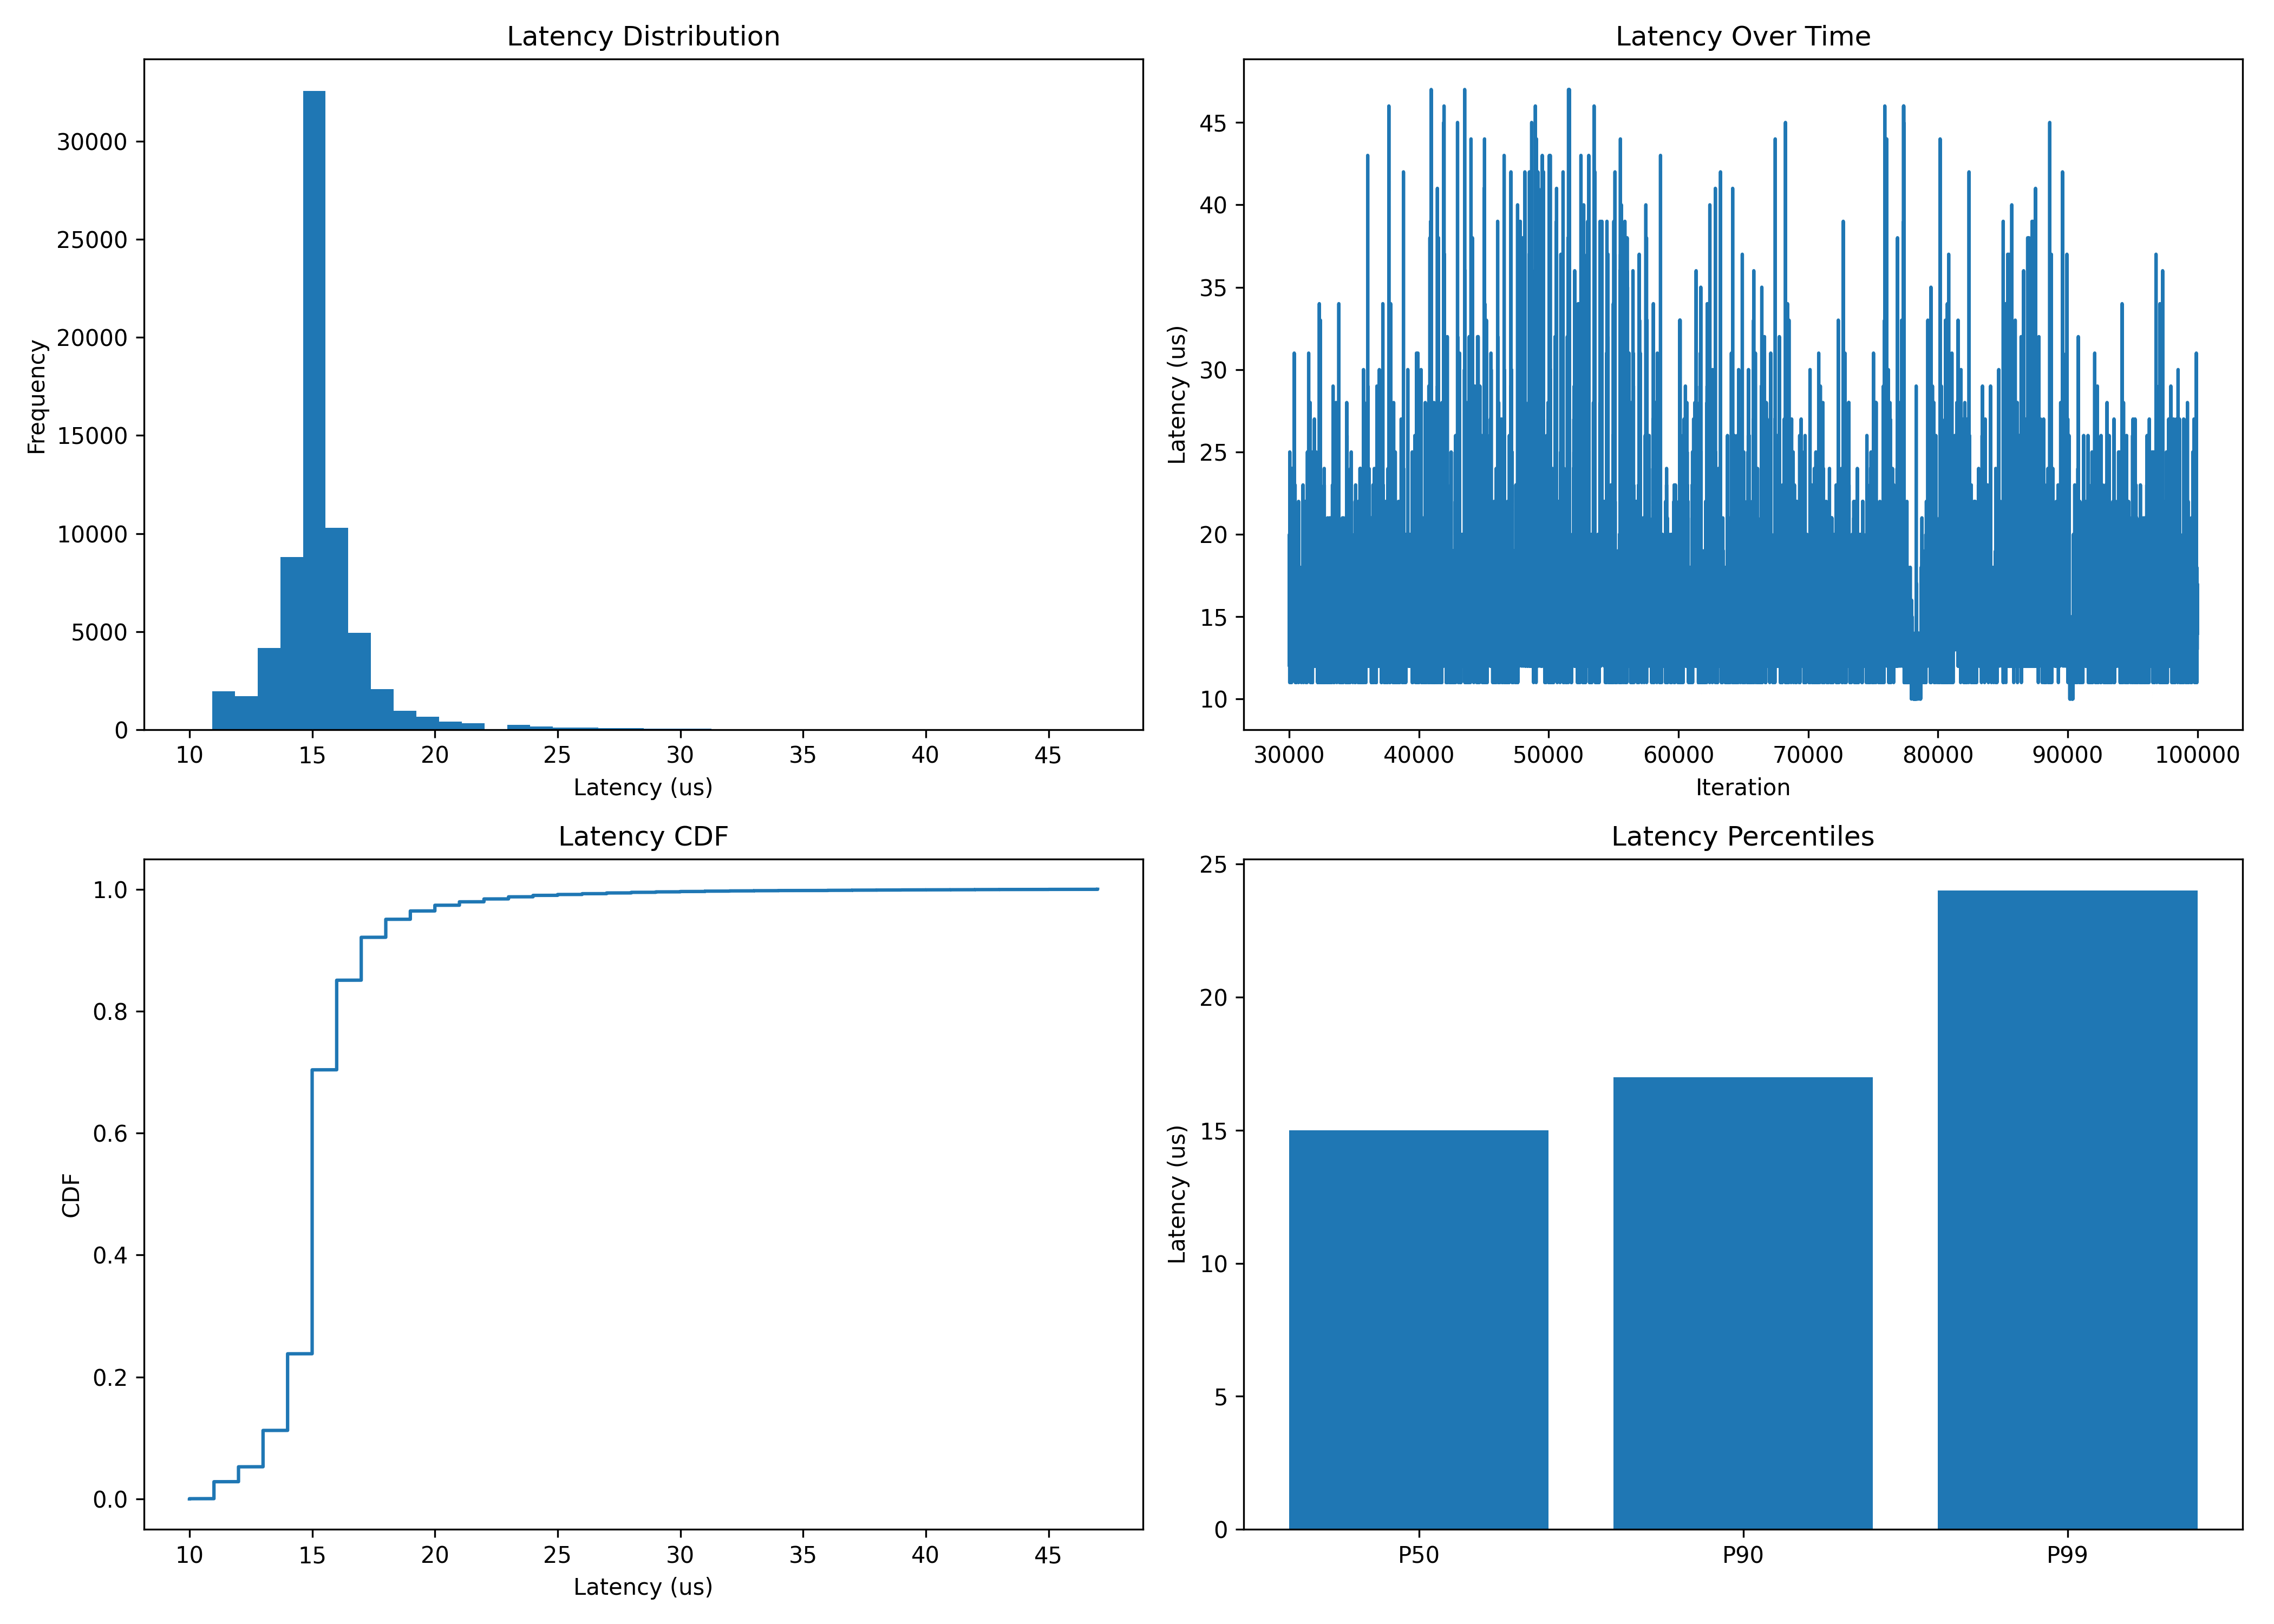
\includegraphics[width=0.85\textwidth]{figures/fig01-latency-analysis.png}
\caption{Latency analysis (first attempt, loopback TCP).}
\label{fig:first-latency}
\end{figure}

\subsection{Flaws in the first implementation}

\begin{itemize}
\item \texttt{priority\_queue} stores orders scattered across the heap.
      Every \texttt{top()} and \texttt{pop()} potentially pulls a different
      cache line from RAM. This introduces cache misses and increases
      latency.
\item String-based message protocol forces heap allocation on every order.
      Operations like \texttt{std::string}, \texttt{stringstream}, and
      string concatenation allocate and free memory dynamically, causing
      unpredictable latency spikes in the hot path.
\item No framing protocol on the TCP stream. TCP delivers a byte stream
      with no message boundaries. A single \texttt{read()} call may return
      multiple concatenated orders or a partial order. Without a
      length-prefix or complete read loop, the parser silently corrupts or
      drops orders under load.
\item Single-threaded blocking design. The server blocks on
      \texttt{accept()} waiting for one client, then blocks on
      \texttt{read()} waiting for each order. There is no concurrency ---
      a slow client stalls the entire matching engine.
\item No error checking on socket operations. \texttt{send()} and
      \texttt{read()} can return partial results or fail silently. The
      implementation assumes every call succeeds and transfers the full
      message, which is not guaranteed by the OS.
\item \texttt{cout} inside the matching hot path. Writing to stdout on
      every order and every trade is a system call that blocks until the
      terminal flushes. This artificially inflates latency measurements and
      would be unacceptable in production.
\item Order book state is unbounded in memory. Unmatched orders accumulate
      in the priority queues indefinitely with no cancellation, expiry, or
      memory reclamation mechanism. Under sustained load the process grows
      without bound.
\item No order cancellation or modification. A real order book must support
      cancel and replace operations. Without them the book fills with stale
      orders that can never be matched or removed.
\end{itemize}

\subsection{Measurement improvement}

The initial benchmark implementation introduced significant overhead due to
repeated terminal output inside the critical request--response path. Both
the client and server were performing \texttt{cout} operations for every
processed order, which resulted in additional system calls, buffering
overhead, synchronization costs, and scheduler interruptions. As a
consequence, the measured latency reflected not only the networking and
matching engine performance, but also terminal I/O overhead.

To obtain a more accurate estimate of the order processing latency, all
logging operations were removed from the hot execution path. After this
optimization, the benchmark was executed for 100{,}000 orders over a
localhost TCP connection on an Apple M1 system.

\begin{table}[h]
\centering
\begin{tabular}{lr}
\toprule
Metric & Latency \\
\midrule
Minimum & 10\,$\mu$s \\
Maximum & 231\,$\mu$s \\
Mean    & 15\,$\mu$s \\
P50     & 15\,$\mu$s \\
P90     & 17\,$\mu$s \\
P99     & 24\,$\mu$s \\
\bottomrule
\end{tabular}
\caption{Round-trip latency after removing logging from the hot path
(100{,}000 orders, Apple M1).}
\end{table}

The reduction in both average latency and tail latency demonstrates the
substantial impact of unnecessary I/O operations on low-latency systems.
Although this benchmark is not a perfectly isolated measurement of the
matching engine itself, it serves as a useful end-to-end latency benchmark
for evaluating future optimizations to the order book implementation. In
particular, it provides a practical baseline for studying the effects of
protocol design, parsing overhead, memory allocation, and networking
optimizations on overall system latency.

\begin{figure}[h]
\centering
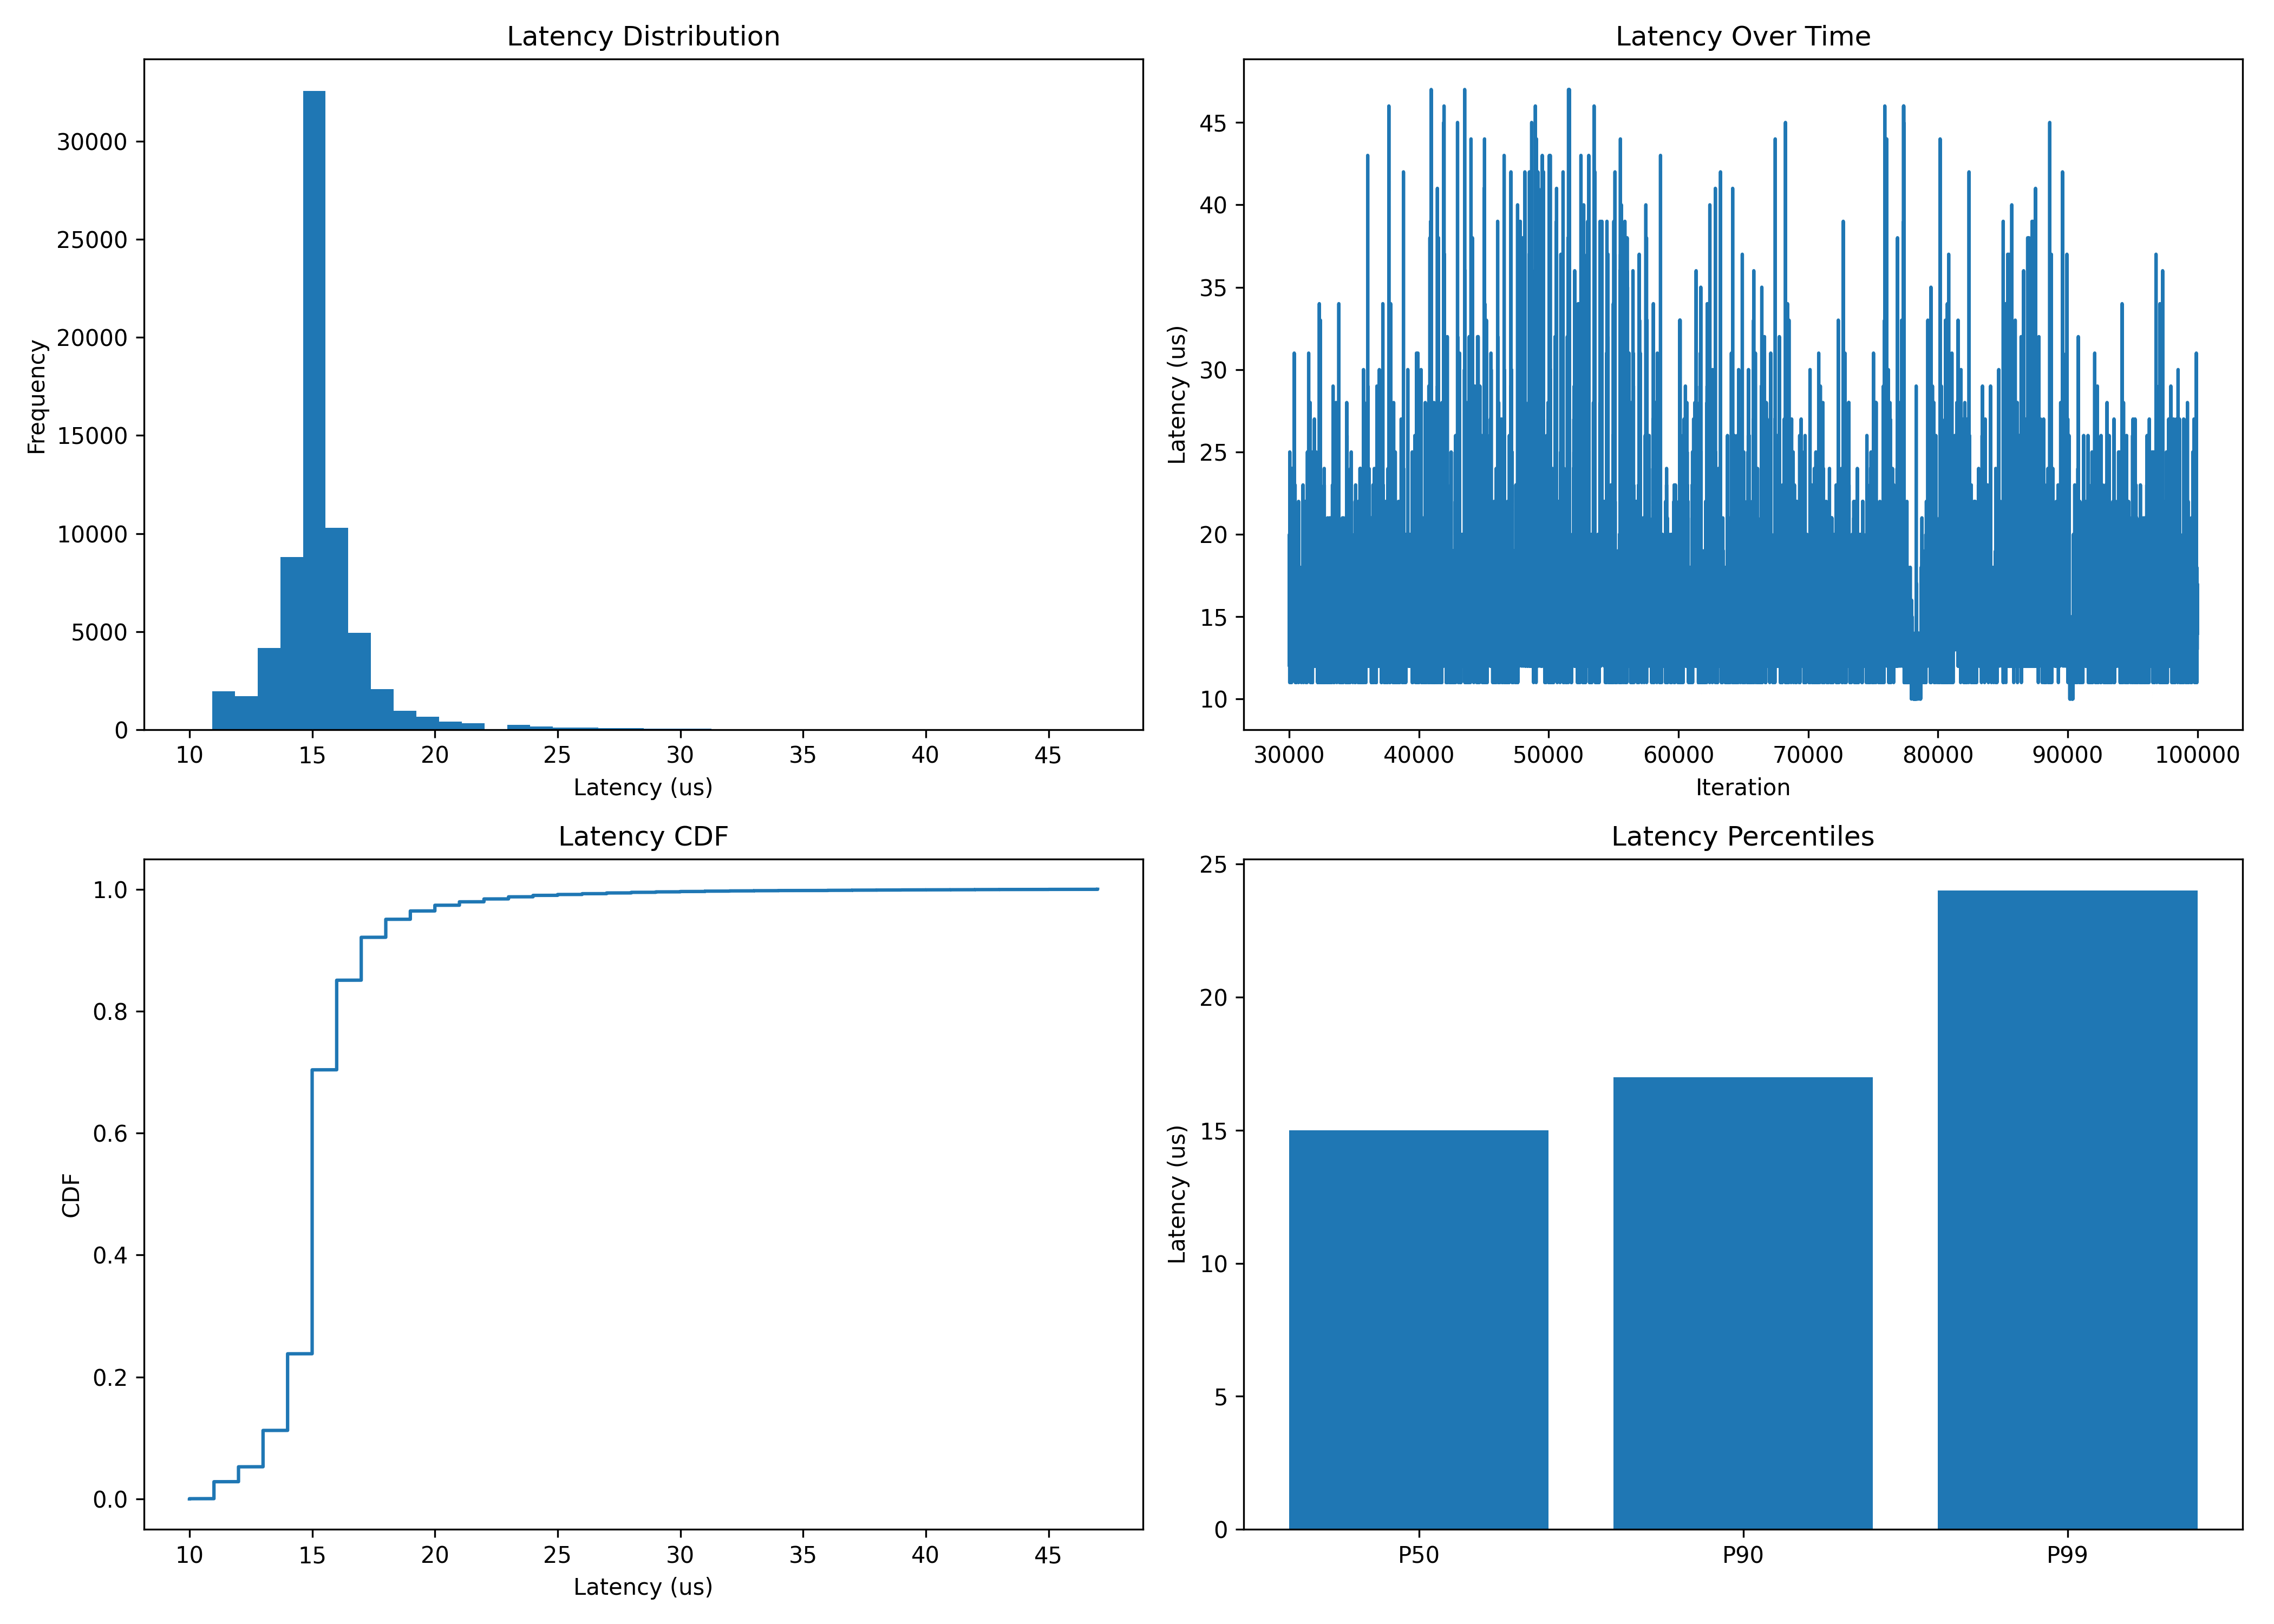
\includegraphics[width=0.85\textwidth]{figures/fig02-latency-clean.png}
\caption{Latency analysis after removing warm-up iterations and extreme
outliers.}
\label{fig:first-clean}
\end{figure}

\section{Second Attempt}\label{sec:second}

\subsection{Order book implementation}

This time the order book was implemented using a price-indexed vector of
price levels, improving cache performance over the prior
\texttt{priority\_queue}-based design, which suffered from the following
limitation:

\begin{itemize}
\item \texttt{priority\_queue} stores orders scattered across the heap.
      Every \texttt{top()} and \texttt{pop()} potentially pulls a different
      cache line from RAM. This introduces cache misses and increases
      latency.
\end{itemize}

Instead, the order book is backed by two flat vectors of
\texttt{PriceLevel} structs, one for bids and one for asks, indexed directly
by price tick.

\begin{lstlisting}[caption={Order book data structures (phase 2)}]
struct PriceLevel {
    queue<uint64_t> orders;   // stores order IDs in FIFO order
    int total_qty = 0;
};

struct OrderBook {
    static const int MIN_PRICE = 0;
    static const int MAX_PRICE = 10000;
    static const int TICK_SIZE = 5;

    vector<PriceLevel> asks;
    vector<PriceLevel> bids;
    unordered_map<uint64_t, Order> order_map;

    int best_bid = INT_MIN;
    int best_ask = INT_MAX;
};
\end{lstlisting}

Each price level maps directly to a vector index via a tick conversion,
giving O(1) access to any price level without heap traversal.

\begin{lstlisting}[caption={Price to index conversion}]
int to_index(int raw_price) {
    if (raw_price > MAX_PRICE || raw_price < MIN_PRICE) return -1;
    return (raw_price - MIN_PRICE) / TICK_SIZE;
}
\end{lstlisting}

Price--time priority is preserved naturally: each \texttt{PriceLevel} holds
a \texttt{queue} of order IDs, so orders at the same price are matched
strictly in FIFO order. The best bid and best ask prices are tracked
explicitly as integers, updated incrementally on each add, cancel, and
match, avoiding any scan in the common case. When a level is exhausted, a
linear scan finds the next occupied level.

\begin{lstlisting}[caption={Matching logic (phase 2)}]
void match() {
    while (best_bid >= best_ask) {
        PriceLevel& bid_level = bids[to_index(best_bid)];
        PriceLevel& ask_level = asks[to_index(best_ask)];

        // skip cancelled orders at front of each level
        while (!bid_level.orders.empty()) {
            auto it = order_map.find(bid_level.orders.front());
            if (it != order_map.end()) break;   // live order
            bid_level.orders.pop();             // zombie: discard
        }
        // ... same for asks ...

        int traded_qty = min(bid.qty, ask.qty);
        bid.qty -= traded_qty;
        ask.qty -= traded_qty;
        bid_level.total_qty -= traded_qty;
        ask_level.total_qty -= traded_qty;

        if (bid.qty == 0) {
            order_map.erase(bid.id);
            bid_level.orders.pop();
        }
        if (ask.qty == 0) {
            order_map.erase(ask.id);
            ask_level.orders.pop();
        }

        if (bid_level.orders.empty())
            best_bid = find_next_bid(to_index(best_bid) - 1);
        if (ask_level.orders.empty())
            best_ask = find_next_ask(to_index(best_ask) + 1);
    }
}
\end{lstlisting}

Since both \texttt{bids} and \texttt{asks} are contiguous vectors, accessing
nearby price levels reuses the same cache lines, eliminating the
pointer-chasing overhead of heap-based traversal. Order lookup and
cancellation are handled via an \texttt{unordered\_map} keyed on order ID,
providing O(1) average-case access. Lazy cancellation is used: cancelled
orders are marked in the map and skipped at match time, avoiding the O(n)
cost of removing an arbitrary element from the middle of a heap.

\subsection{Measurement bottleneck and direct benchmarking}

The initial benchmarking strategy was designed to simulate a realistic
deployment environment, where orders were transmitted over a TCP socket and
latency was measured as the full round-trip time between transmission and
acknowledgement. However, this methodology produced nearly identical
results for both implementations, with average latencies of approximately
15\,$\mu$s in each case.

This similarity was not due to architectural equivalence between the two
order book designs. Instead, the dominant cost originated from the
networking stack itself. The loopback TCP round-trip --- including kernel
context switches, socket buffer management, and the \texttt{read}/
\texttt{write} system calls --- contributed roughly 14--15\,$\mu$s per
operation. As a result, the actual order book processing time, which
occurred entirely in userspace, accounted for less than 5\% of the measured
latency.

Consequently, any performance difference between the two data structures
became indistinguishable at microsecond resolution.

To isolate the performance of the matching engines themselves, both
implementations were subsequently benchmarked entirely in-process,
eliminating all networking and IPC overhead. Orders were pre-generated
before entering the timed region in order to exclude random number
generation costs. Each individual \texttt{add\_order()} invocation was then
measured independently using \texttt{chrono::high\_resolution\_clock} at
nanosecond resolution. The resulting measurements are:

\begin{table}[h]
\centering
\begin{tabular}{lrr}
\toprule
Metric & Priority queue & Vector + hash map \\
\midrule
Mean (filtered) & 212.9 ns & 174.1 ns \\
P50             & 83 ns    & 84 ns    \\
P90             & 542 ns   & 375 ns   \\
P99             & 917 ns   & 791 ns   \\
\bottomrule
\end{tabular}
\caption{Per-order in-process latency measurements after outlier filtering
(Apple M1, \texttt{high\_resolution\_clock} brackets).}
\label{tab:phase12}
\end{table}

The vector-based implementation demonstrates an approximately 18\% reduction
in mean latency and a 31\% reduction at the P90 percentile relative to the
priority queue implementation. The P50 values remain nearly identical,
indicating that both implementations process simple non-matching insertions
with similar efficiency.

The divergence becomes more pronounced at higher percentiles, particularly
at P90 and P99, which is consistent with the expected algorithmic behaviour
of the two approaches. In the priority queue implementation, order matching
requires repeated heap restructuring operations during \texttt{match()},
each incurring O(log n) comparisons together with poor cache locality due to
pointer-heavy heap traversal. In contrast, the vector-based implementation
accesses contiguous memory regions corresponding to price levels and
determines the best price through direct integer indexing, thereby avoiding
heap traversal entirely.

As a result, the vector-based design exhibits significantly lower tail
latency under heavy matching pressure, where the cache penalties and
repeated restructuring costs of the priority queue accumulate across
multiple \texttt{push()} and \texttt{pop()} operations.

\begin{revision}
Table~\ref{tab:phase12} percentiles were computed \emph{after} a
Tukey-fence outlier filter, and the measurement bracket cost
(two vDSO clock calls) is a substantial fraction of the P50. The
\emph{relative} conclusion --- the vector design wins the tail --- is
correct and was re-confirmed by the reference-book measurement of
Section~\ref{sec:sixth} on a per-phase basis.
\end{revision}

\section{Third Attempt}\label{sec:third}

\subsection{Inspiration and architectural shift}

For the third iteration of the matching engine, significant architectural
inspiration was drawn from the open-source C++ \texttt{OrderBook}
implementation by Coding Jesus. While the second attempt successfully
isolated the matching engine from network overhead and demonstrated the raw
speed of contiguous memory layouts, it ultimately optimized for a very
specific, narrow-tick market. To build a robust, production-ready system
capable of handling advanced order types, sparse liquidity, and massive
cancellation volumes, a fundamental shift in data structures was required.

\subsection{Evaluating the second implementation}

Before detailing the new architecture, we analyze the theoretical and
practical limitations of the vector-based approach developed in phase 2.

\paragraph{Pros of the vector implementation}
\begin{itemize}
\item \textbf{Cache locality.} Storing price levels in a contiguous
      \texttt{std::vector} heavily leveraged CPU prefetching, practically
      eliminating the pointer-chasing overhead seen in the initial priority
      queue implementation.
\item \textbf{O(1) indexing.} Mapping a raw price directly to a vector
      index provided mathematically optimal constant-time access to any
      known price level.
\end{itemize}

\paragraph{Cons and structural flaws}
\begin{itemize}
\item \textbf{Sparse book degradation.} If a price level was exhausted,
      finding the next available best bid or ask required a linear array
      scan (\texttt{find\_next\_bid()}). In a sparse market (e.g.\ options
      or high-volatility crypto) where the spread might instantly widen by
      thousands of ticks, this O(N) scan would completely destroy
      microsecond latency.
\item \textbf{Lazy cancellation bloat.} Because \texttt{std::queue} does not
      support middle-element removal, cancelled orders were simply flagged
      in a hash map and left in the queue. In modern markets where upward of
      90\% of orders are cancelled before execution, this lazy approach
      causes unbounded memory bloat. Furthermore, it forces the matching
      loop to waste CPU cycles checking and popping zombie orders during
      active trading.
\end{itemize}

\subsection{Inherited architecture and theoretical superiority}

To resolve these bottlenecks, this third implementation adopts a more
dynamic topology, prioritizing immediate state resolution over raw array
density. The core data structures inherited from the Coding Jesus
architecture are:

\begin{itemize}
\item \textbf{Price levels via red--black tree (\texttt{std::map}).} Instead
      of a flat vector, bids and asks are maintained in a \texttt{std::map}
      keyed by price. While finding a specific price level now incurs an
      O(log M) cost (where M is the number of active price levels), finding
      the \emph{next} best price when a level is exhausted is an O(1)
      operation via a simple iterator increment. This makes the engine
      effectively immune to spread widening in sparse markets.
\item \textbf{Time priority via doubly-linked list (\texttt{std::list}).}
      Orders at a specific price level are maintained in a
      \texttt{std::list} rather than a \texttt{std::queue}.
\item \textbf{True O(1) immediate cancellation.} By storing the exact
      \texttt{std::list::iterator} alongside the order details inside an
      \texttt{std::unordered\_map}, an order can be instantly erased from
      the middle of the linked list in absolute O(1) time.
\end{itemize}

\subsection{Quantitative expectation}

From a quantitative perspective, this architectural pivot trades a slightly
higher baseline insertion cost for heavily suppressed tail latencies during
market turbulence. In the phase 2 implementation, the cost of handling
cancellations was deferred to the \texttt{match()} function. If a sudden
market movement triggered 1{,}000 cancellations, the next incoming market
order would bear the O(K) latency penalty of popping those 1{,}000 dead
orders before finding actionable liquidity.

By enforcing true O(1) immediate cancellation, the phase 3 architecture
guarantees that the \texttt{match()} loop only ever interacts with live,
executable liquidity. While the P50 insertion latency is expected to
slightly increase due to the O(log M) tree traversal and dynamic node
allocation, the P90 and P99 latencies during heavy cancel-to-trade
intervals should demonstrate massive stabilization.

\subsection{Implementation details}

The core structures: the book is a pair of \texttt{std::map}s keyed by
price; each \texttt{PriceLevel} holds a FIFO \texttt{std::list} of order
IDs and the aggregate quantity; a central registry
(\texttt{unordered\_map}) stores, for every live order, its full
\texttt{Order} value together with a stable \texttt{map} iterator to its
level and a stable \texttt{list} iterator to its position, so both matching
and cancellation are direct iterator operations.

\begin{lstlisting}[caption={Phase 3 order book data structures
(\texttt{orderbook.h})}]
enum class Side { BID, ASK };
enum class OrderType { LIMIT, MARKET };

struct Order {
    uint64_t id;
    Side side;
    int price;
    int qty;
    OrderType type;
};

struct PriceLevel {
    std::list<uint64_t> orders;  // FIFO: front = highest priority
    int total_qty = 0;
};

struct OrderMeta {
    Order order;
    std::map<int, PriceLevel>::iterator level_it; // O(1) level handle
    std::list<uint64_t>::iterator order_it;       // O(1) position handle
};

struct TradeReport {
    uint64_t bid_id;
    uint64_t ask_id;
    int price;
    int qty;
};

class OrderBook {
public:
    std::vector<TradeReport> add_order(const Order& order);
    bool cancel_order(uint64_t order_id);
    int best_bid() const;
    int best_ask() const;

private:
    std::map<int, PriceLevel> bids_;  // sorted ascending; best = rbegin()
    std::map<int, PriceLevel> asks_;  // sorted ascending; best = begin()
    std::unordered_map<uint64_t, OrderMeta> order_map_;

    void insert_limit(const Order& order);
    std::vector<TradeReport> match(Side taker_side);
    void remove_level_if_empty(Side side,
        std::map<int, PriceLevel>::iterator it);
};
\end{lstlisting}

The execution logic highlights how the matching and cancellation loops
remain clean of dead elements, completely bypassing the zombie-scanning
overhead seen in the phase 2 lazy-cancellation design.

\begin{lstlisting}[caption={Phase 3 insertion and immediate cancellation
(\texttt{orderbook.cpp})}]
void OrderBook::insert_limit(const Order& order) {
    auto& book = (order.side == Side::BID) ? bids_ : asks_;
    auto level_it = book.emplace(order.price, PriceLevel{}).first;
    PriceLevel& level = level_it->second;

    level.total_qty += order.qty;
    level.orders.push_back(order.id);

    OrderMeta meta;
    meta.order    = order;
    meta.level_it = level_it;
    meta.order_it = std::prev(level.orders.end());
    order_map_.emplace(order.id, std::move(meta));
}

bool OrderBook::cancel_order(uint64_t order_id) {
    auto it = order_map_.find(order_id);
    if (it == order_map_.end()) return false;

    OrderMeta& meta = it->second;
    PriceLevel& level = meta.level_it->second;

    level.total_qty -= meta.order.qty;
    level.orders.erase(meta.order_it);   // true O(1) removal

    remove_level_if_empty(meta.order.side, meta.level_it);
    order_map_.erase(it);
    return true;
}
\end{lstlisting}

\begin{lstlisting}[caption={Phase 3 matching logic
(\texttt{orderbook.cpp})}]
std::vector<TradeReport> OrderBook::match(Side taker_side) {
    std::vector<TradeReport> reports;
    while (!bids_.empty() && !asks_.empty()) {
        auto bid_level_it = std::prev(bids_.end());
        auto ask_level_it = asks_.begin();

        if (bid_level_it->first < ask_level_it->first) break;

        PriceLevel& bid_level = bid_level_it->second;
        PriceLevel& ask_level = ask_level_it->second;

        while (!bid_level.orders.empty() && !ask_level.orders.empty()) {
            uint64_t bid_id = bid_level.orders.front();
            uint64_t ask_id = ask_level.orders.front();

            OrderMeta& bid_meta = order_map_.at(bid_id);
            OrderMeta& ask_meta = order_map_.at(ask_id);

            int trade_price = (taker_side == Side::BID)
                                  ? ask_level_it->first
                                  : bid_level_it->first;
            int traded_qty  = std::min(bid_meta.order.qty,
                                       ask_meta.order.qty);

            bid_meta.order.qty -= traded_qty;
            ask_meta.order.qty -= traded_qty;
            bid_level.total_qty -= traded_qty;
            ask_level.total_qty -= traded_qty;

            reports.push_back({bid_id, ask_id, trade_price, traded_qty});

            if (bid_meta.order.qty == 0) {
                bid_level.orders.pop_front();
                order_map_.erase(bid_id);
            }
            if (ask_meta.order.qty == 0) {
                ask_level.orders.pop_front();
                order_map_.erase(ask_id);
            }
        }
        remove_level_if_empty(Side::BID, bid_level_it);
        remove_level_if_empty(Side::ASK, ask_level_it);
    }
    return reports;
}
\end{lstlisting}

\subsection{Workload stress testing and workload divergence}

To properly evaluate the architectural trade-offs between continuous
indexing (phase 2) and pointer-based structural logic (phase 3), the
benchmark framework implements two distinct, high-fidelity synthetic
workloads:

\begin{itemize}
\item \textbf{Dense workload.} 300{,}000 operations over a narrow, tightly
      clustered price band (9{,}900 to 10{,}100). This guarantees that price
      levels are highly populated and continuously reused, directly
      favoring contiguous buffer strategies.
\item \textbf{Sparse workload.} 150{,}000 operations distributed across an
      expansive price frontier spanning 200{,}000 possible ticks, organized
      into 20 isolated micro-clusters. This creates massive liquidity
      voids. When a price level is cleared out during heavy matching or
      aggressive cancellations, the engine is forced to locate the next
      active resting level across vast spans of empty space.
\end{itemize}

Both scenarios integrate a heavy 40\% cancel-to-order ratio to stress-test
immediate versus deferred element reclamation under fire.

\subsection{Empirical data analysis and plot interpretation}

The empirical benchmarks collected on an Apple Silicon environment confirm
the low-latency algorithmic trade-offs. The system performance across both
workloads breaks down as follows:

\begin{table}[h]
\centering
\begin{tabular}{lrrrr}
\toprule
Phase (structure) & \multicolumn{2}{c}{Dense} & \multicolumn{2}{c}{Sparse} \\
\cmidrule(lr){2-3}\cmidrule(lr){4-5}
 & Mean & P99 & Mean & P99 \\
\midrule
1 --- priority queue   & 42.5\,ns  & 167\,ns & ---        & ---      \\
2 --- tick vector      & 58.3\,ns  & 209\,ns & 2{,}165\,ns & 33{,}583\,ns \\
3 --- map + list       & 120.9\,ns & 500\,ns & 113.2\,ns  & 459\,ns  \\
\bottomrule
\end{tabular}
\caption{Historical phase 1--3 results (Apple M1,
\texttt{high\_resolution\_clock}, Tukey-filtered). Reproduced from the
original notebook; see the revision note in Section~\ref{sec:intro}.}
\label{tab:phase123}
\end{table}

\subsubsection{The dense micro-benchmark verdict}

Under dense market conditions, phase 1 (priority queue) and phase 2 (tick
vector) exhibit tight execution profiles, posting mean latencies of
42.5\,ns and 58.3\,ns respectively, with P99 tail latencies capping out near
167\,ns and 209\,ns.

Phase 3 (map + list) records a mean latency of 120.9\,ns and a P99 of
500\,ns. This variance is visually captured in the grouped bar chart
(percentile comparison) and the dense distribution graph (histogram), where
the phase 3 curve shifts noticeably to the right.

This behavior represents the pure cost of hardware-level non-locality: the
\texttt{std::map} structure forces dynamic node allocation upon insertion,
causing pointer-chasing across the heap during traversal, while
\texttt{std::list} introduces additional reference linkages that degrade
L1/L2 cache efficiency relative to contiguous vector slots.

Interestingly, the add-vs-cancel plot reveals a hidden structural strength
of phase 3: its cancellation latency remains perfectly uniform and identical
to its insertion latency (around 33\,ns). Because it relies on true direct
iterator execution, removing a resting order from the center of the list
skips the matching logic entirely and completes in pure, predictable
constant time.

\begin{figure}[h]
\centering
\begin{subfigure}{0.48\textwidth}
    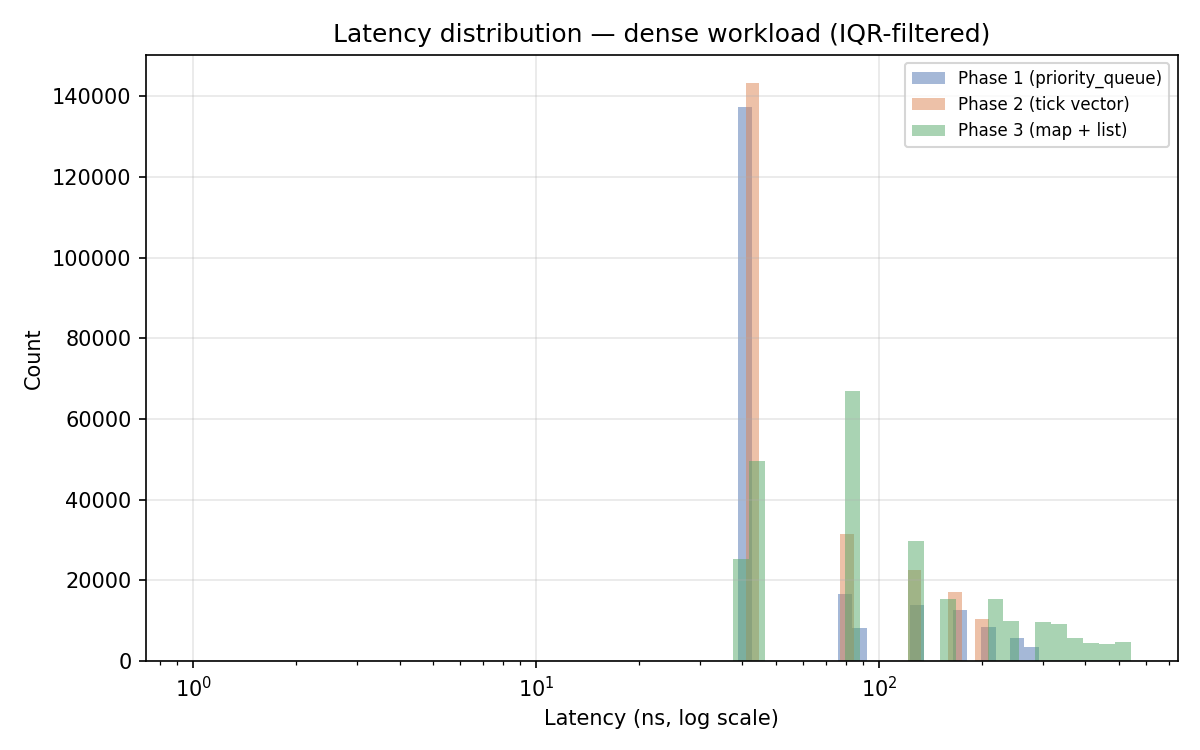
\includegraphics[width=\textwidth]{figures/fig03a-histogram-dense.png}
    \caption{Dense latency distribution.}
\end{subfigure}
\hfill
\begin{subfigure}{0.48\textwidth}
    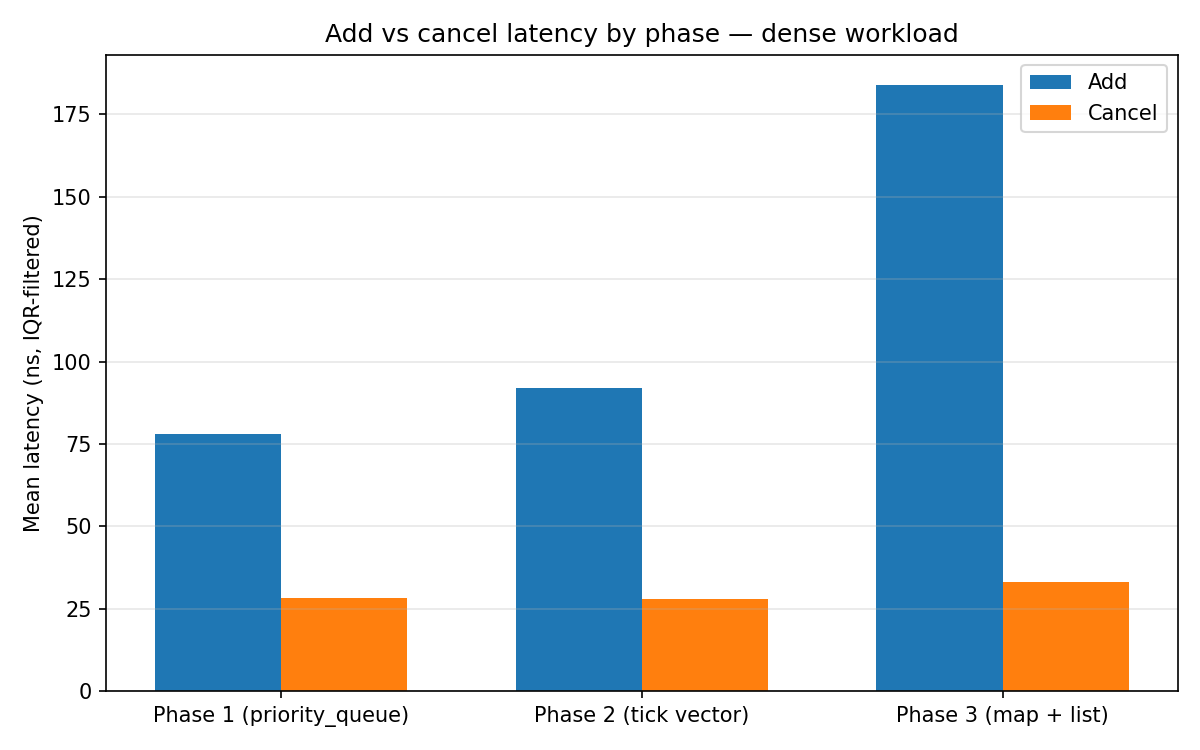
\includegraphics[width=\textwidth]{figures/fig03b-add-vs-cancel.png}
    \caption{Add vs.\ cancel latency.}
\end{subfigure}
\caption{Phase 3 performance benchmarks under dense workloads
(historical, Apple M1).}
\label{fig:phase3-dense}
\end{figure}

\subsubsection{The sparse micro-benchmark catastrophe}

When switched to the sparse market configuration, the structural flaws of
phase 2 explode mathematically. The mean latency for phase 2 surges from
58.3\,ns to an unviable 2{,}165\,ns, while its P99 tail latency shoots up to
33{,}583\,ns.

The root cause of this operational collapse is diagnosed by the log-scale
time series plots and the cumulative probability curves. The phase 2 curve
stretches out into a massive high-latency tail plateau between $10^4$ and
$10^5$\,ns. Whenever a price cluster is cleared out, phase 2 executes a flat
linear loop (\texttt{find\_next\_bid}/\texttt{find\_next\_ask}) scanning
across thousands of empty array coordinates. In stark contrast, phase 3
remains entirely stable, posting a steady mean latency of 113.2\,ns and a
rock-solid P99 tail of 459\,ns. Because \texttt{std::map} holds active price
levels inside a balanced red--black tree, moving to the next best available
price level is an O(1) pointer increment on the iterator. The engine
completely bypasses the empty space, proving its total immunity to wide
spreads and volatile liquidity drops.

\begin{figure}[h]
\centering
\begin{subfigure}{0.48\textwidth}
    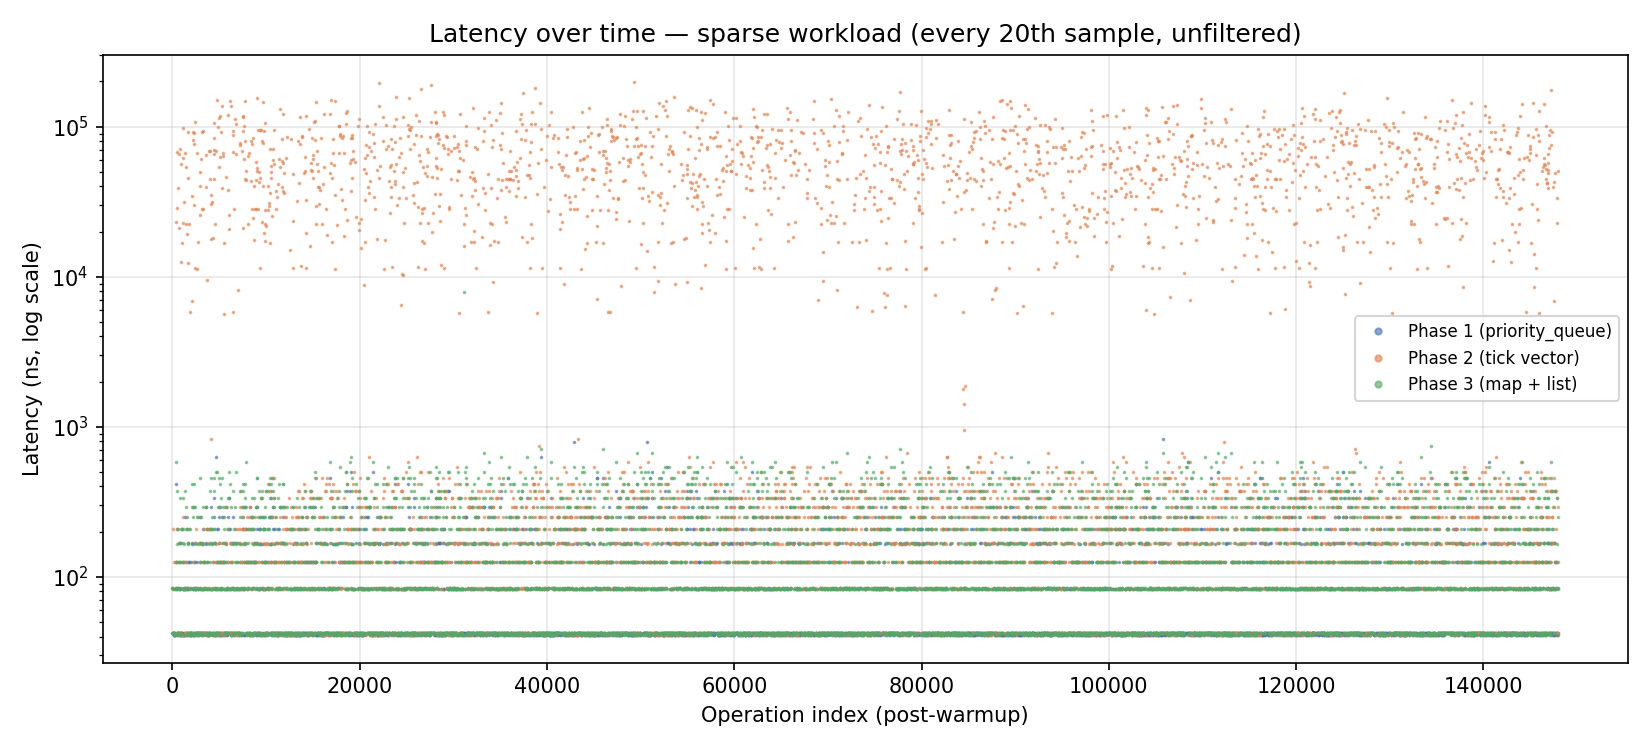
\includegraphics[width=\textwidth]{figures/fig04a-timeseries-sparse.png}
    \caption{Sparse latency over time.}
\end{subfigure}
\hfill
\begin{subfigure}{0.48\textwidth}
    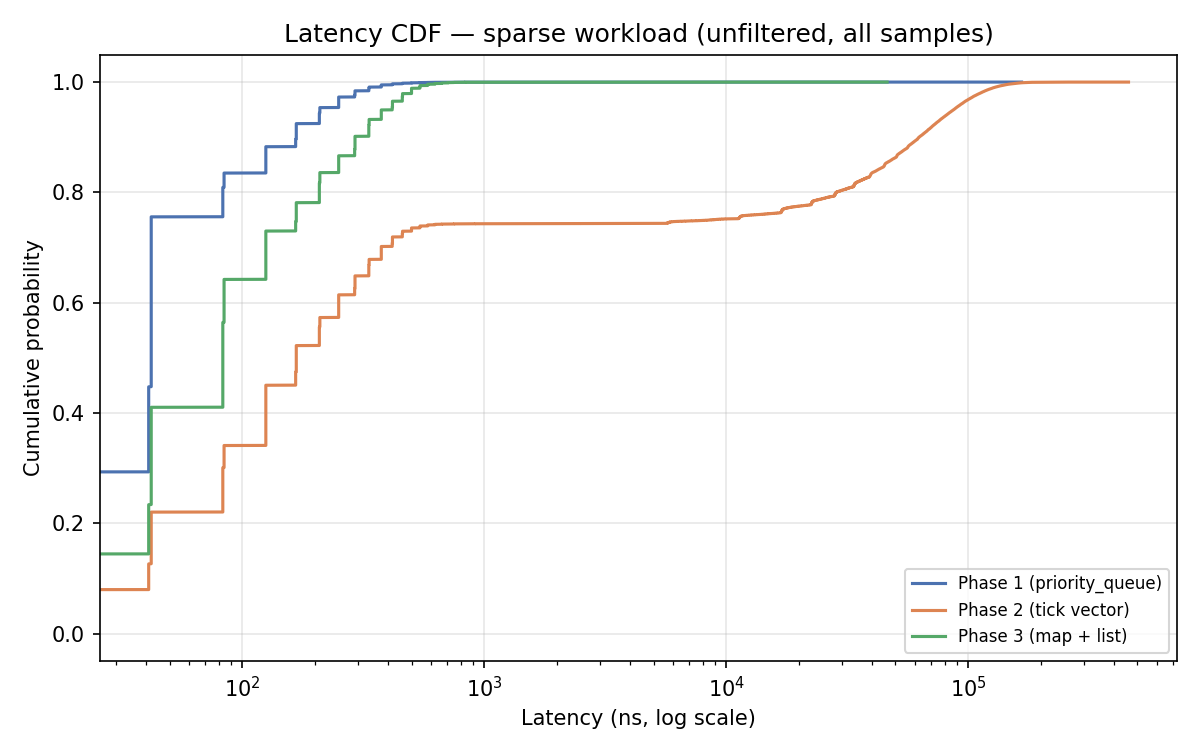
\includegraphics[width=\textwidth]{figures/fig04b-cdf-sparse.png}
    \caption{Empirical CDF (sparse).}
\end{subfigure}
\caption{Phase 2 vs.\ phase 3 behavior under sparse workloads
(historical, Apple M1).}
\label{fig:phase3-sparse}
\end{figure}

\begin{figure}[h]
\centering
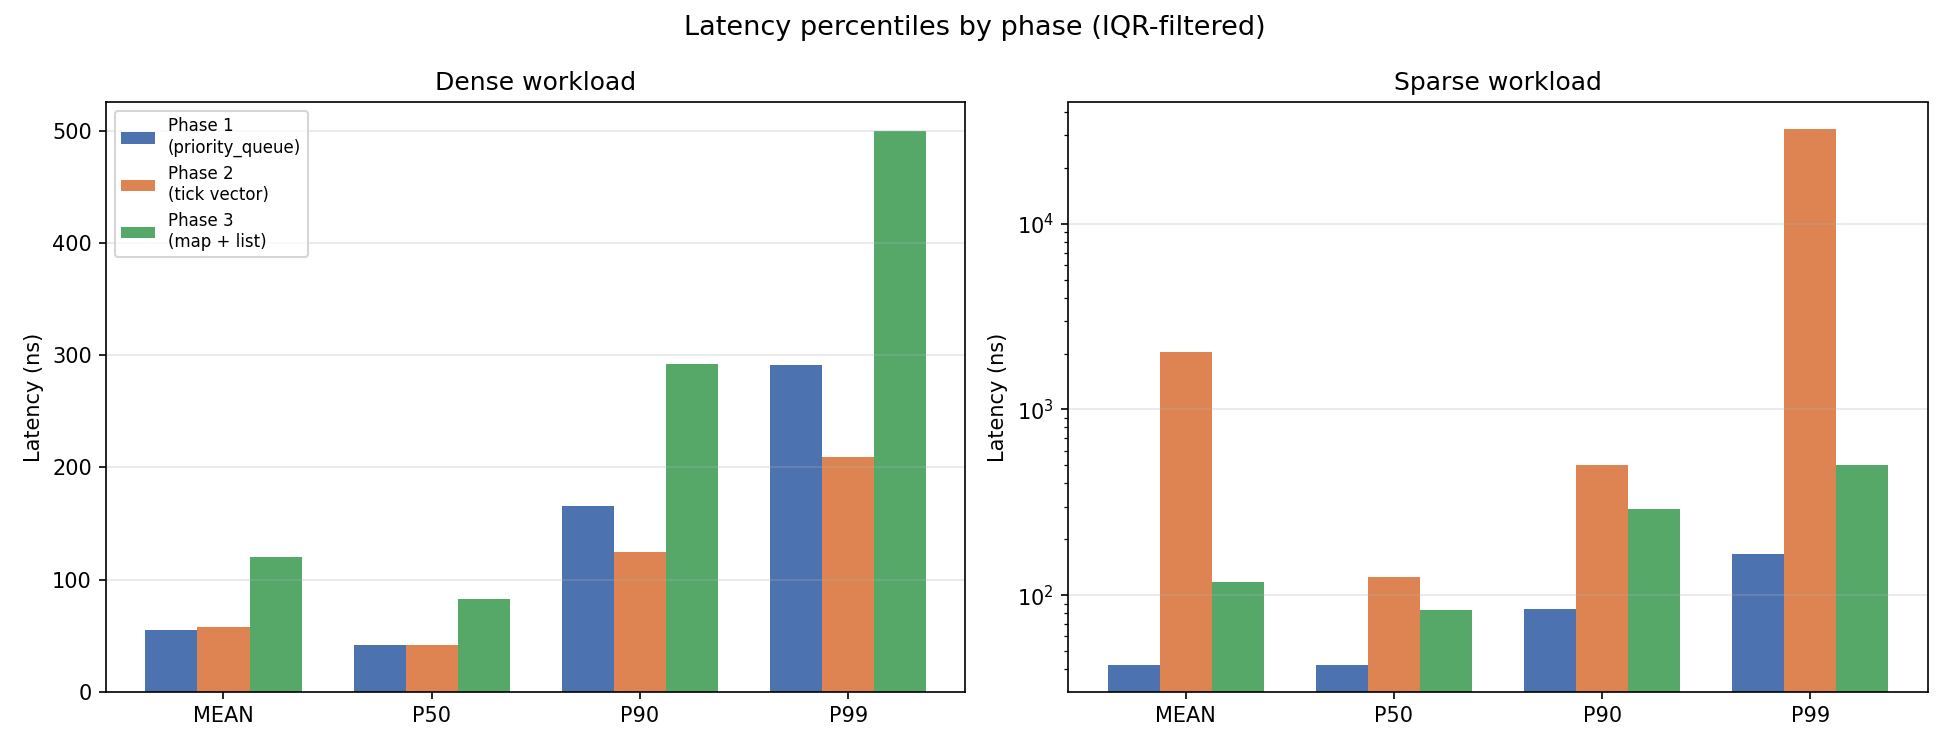
\includegraphics[width=0.95\textwidth]{figures/fig05-percentile-comparison.png}
\caption{Grouped percentile comparison (mean, P50, P90, P99) between all
three phases across dense and sparse workloads (historical, Apple M1).}
\label{fig:phase123-compare}
\end{figure}

\section{Fourth Attempt: The Middle Ground}\label{sec:fourth}

\subsection{The hardware vs.\ logic dilemma}

Phases 2 and 3 exposed a clean trade-off: contiguous arrays are
hardware-fast but algorithmically fragile in sparse books; pointer-based
trees are algorithmically robust but hardware-slow. Phase 4 asks whether the
\emph{structure} of the book can keep array-grade memory locality while
regaining the algorithmic guarantees --- O(1) cancellation and O(log-levels)
price discovery --- that the tree provided for free.

\subsection{Solving the sparse book: bitmask array}

The flat level array is retained, but the search for the next occupied tick
is no longer a linear scan. A \texttt{TickBitset} keeps one bit per price
tick; finding the best price becomes a count-trailing-zeros
(\texttt{\_\_builtin\_ctzll}) / count-leading-zeros operation over 64-bit
words --- one instruction per 64 ticks.

\begin{lstlisting}[caption={Bitmask next-price discovery (phase 4)}]
int find_next_set(int from_idx) {
    size_t word = from_idx >> 6;
    uint64_t w = words_[word] & (~0ULL << (from_idx & 63));
    if (w) return word * 64 + __builtin_ctzll(w);

    for (size_t i = word + 1; i < words_.size(); ++i) {
        if (words_[i] != 0)
            return (i * 64) + __builtin_ctzll(words_[i]);
    }
    return -1;
}
\end{lstlisting}

\subsection{Solving cancellation: memory pools and intrusive lists}

Phase 3 bought O(1) cancellation with \texttt{std::list} node allocation.
Phase 4 keeps the O(1) unlink but removes the allocator: all order nodes
live in one pre-allocated \texttt{std::vector} (a pool). Each node stores
\texttt{next}/\texttt{prev} as \emph{pool indices}, and each price level
stores the pool index of its FIFO head and tail. Cancellation unlinks the
node in constant time and returns it to a free list. An
\texttt{unordered\_map} maps order IDs to pool indices.

\begin{lstlisting}[caption={Intrusive list inside a memory pool (phase 4)}]
struct PriceLevel {
    int32_t head_idx = -1;
    int32_t tail_idx = -1;
    int     total_qty = 0;
};

struct OrderNode {
    uint64_t order_id;
    Side     side;
    int      price;
    int      qty;
    int32_t  price_idx;
    int32_t  next_idx;
    int32_t  prev_idx;
};

// The book:
std::vector<PriceLevel> bid_levels_, ask_levels_; // one per tick
std::vector<OrderNode>  pool_;                    // the memory pool
std::vector<int32_t>    free_list_;               // recycled nodes
std::unordered_map<uint64_t,int32_t> id_to_pool_idx_;
\end{lstlisting}

\subsection{Expected quantitative performance}

The design goal was to keep phase 2's dense-market numbers (its memory
layout is essentially unchanged) while inheriting phase 3's algorithmic
immunity to sparsity --- and to do so with zero heap traffic after
construction.

\subsection{Implementation details}

The bitset write path is fully branchless (two unconditional ORs), the
level arrays are plain \texttt{std::vector<PriceLevel>} indexed by
\texttt{price - price\_min}, and matching walks only the heads of the two
crossed levels, unlinking filled nodes exactly like a cancellation.

\begin{lstlisting}[caption={Hardware-accelerated tick bitset (phase 4)}]
inline void set(int idx) {
    words_[idx >> 6] |= (1ULL << (idx & 63));
}
inline void clear(int idx) {
    words_[idx >> 6] &= ~(1ULL << (idx & 63));
}
inline bool test(int idx) const {
    return (words_[idx >> 6] >> (idx & 63)) & 1ULL;
}
\end{lstlisting}

\begin{lstlisting}[caption={Intrusive list and memory pool initialization
(phase 4)}]
OrderBook::OrderBook(int price_min, int price_max, size_t pool_capacity)
    : price_min_(price_min), price_max_(price_max),
      n_levels_(price_max - price_min + 1),
      bid_levels_(n_levels_), ask_levels_(n_levels_),
      bid_active_(n_levels_), ask_active_(n_levels_),
      pool_(pool_capacity)
{
    free_list_.reserve(pool_capacity);
    for (size_t i = pool_capacity; i-- > 0; )
        free_list_.push_back(static_cast<int32_t>(i));
    id_to_pool_idx_.reserve(pool_capacity);
}
\end{lstlisting}

\begin{lstlisting}[caption={O(1) memory pool cancellation (phase 4)}]
bool OrderBook::cancel_order(uint64_t order_id) {
    auto it = id_to_pool_idx_.find(order_id);
    if (it == id_to_pool_idx_.end()) return false;

    int32_t node_idx = it->second;
    OrderNode& node = pool_[node_idx];
    PriceLevel& level = levels[node.price_idx];

    // O(1) unlink from the intrusive doubly-linked list
    if (node.prev_idx != -1)
        pool_[node.prev_idx].next_idx = node.next_idx;
    else
        level.head_idx = node.next_idx;

    if (node.next_idx != -1)
        pool_[node.next_idx].prev_idx = node.prev_idx;
    else
        level.tail_idx = node.prev_idx;

    id_to_pool_idx_.erase(it);
    free_node(node_idx);   // returns index to free_list_
    return true;
}
\end{lstlisting}

\subsection{Measurement and final results}

The phase 4 architecture was subjected to the exact same dense and sparse
micro-benchmarks as phases 2 and 3. The empirical results confirm that
combining strict contiguous memory mapping with hardware-level bitwise
operations yields major performance improvements in dense markets, but also
reveal a critical bottleneck when navigating extreme sparsity.

\begin{table}[h]
\centering
\begin{tabular}{lrrrr}
\toprule
Workload & Mean & P50 & P90 & P99 \\
\midrule
Dense (narrow tick)  & 56.02\,ns  & 42\,ns & 166\,ns & 250\,ns \\
Sparse (wide tick)   & 105.34\,ns & 42\,ns & 417\,ns & 667\,ns \\
\bottomrule
\end{tabular}
\caption{Phase 4 performance benchmarks (Apple M1,
\texttt{high\_resolution\_clock}, Tukey-filtered).}
\label{tab:phase4}
\end{table}

\paragraph{Dense market analysis.} Under densely populated conditions,
phase 4 achieved a mean latency of 56.02\,ns, effectively matching the raw
execution speed of the pure array-based phase 2 (58.3\,ns). However, it
completely erased the lazy-cancellation bloat. Because node allocation is
bypassed entirely, the median latency dropped to 42\,ns, while the P99 tail
latency remained tightly compressed at 250\,ns, vastly outperforming the
phase 3 tree/list architecture (500\,ns). In tightly packed markets, the
hardware-sympathetic memory pool dominates.

\paragraph{Sparse market analysis.} While phase 4 maintained an exceptional
median latency (42\,ns) under sparse conditions, its performance degraded
significantly at the tail percentiles. At P90 (417\,ns) and P99 (667\,ns),
phase 4 actually underperformed the phase 3 tree/list architecture (292\,ns
and 459\,ns respectively). This indicates that while standard operations
remain blistering fast, the engine struggles severely when forced to
navigate massive liquidity voids.

\subsection{Diagnosing the sparse bottleneck: linear word scanning}

The spike in P90 and P99 latencies under the sparse workload reveals a
subtle structural flaw in the phase 4 \texttt{TickBitset} implementation.

The sparse benchmark spans a massive tick range of 200{,}000 prices. To
represent this, the \texttt{TickBitset} allocates
$\lceil 200{,}000/64 \rceil = 3{,}125$ individual 64-bit words. When the
engine executes \texttt{\_\_builtin\_ctzll}, it finds the next active tick
within a single word in true O(1) time.

However, when a large price void occurs, the engine executes a linear
\texttt{for} loop to find the next non-zero word:

\begin{lstlisting}[caption={The bottleneck: linear scanning over bitmask
words (phase 4)}]
for (size_t i = word_idx + 1; i < words_.size(); ++i) {
    if (words_[i] != 0) {
        return (i * 64) + __builtin_ctzll(words_[i]);
    }
}
\end{lstlisting}

While checking a 64-bit integer against zero is exceptionally fast,
sequentially looping through hundreds of empty words in userspace
re-introduces the exact O(N) penalty that crippled phase 2. During extreme
market volatility where the spread widens significantly, this linear scan
creates the latency spikes observed in the P99 metrics. Phase 3 avoids this
penalty entirely because its \texttt{std::map} iterator skips empty price
space organically via tree traversal.

\begin{figure}[h]
\centering
\begin{subfigure}{0.48\textwidth}
    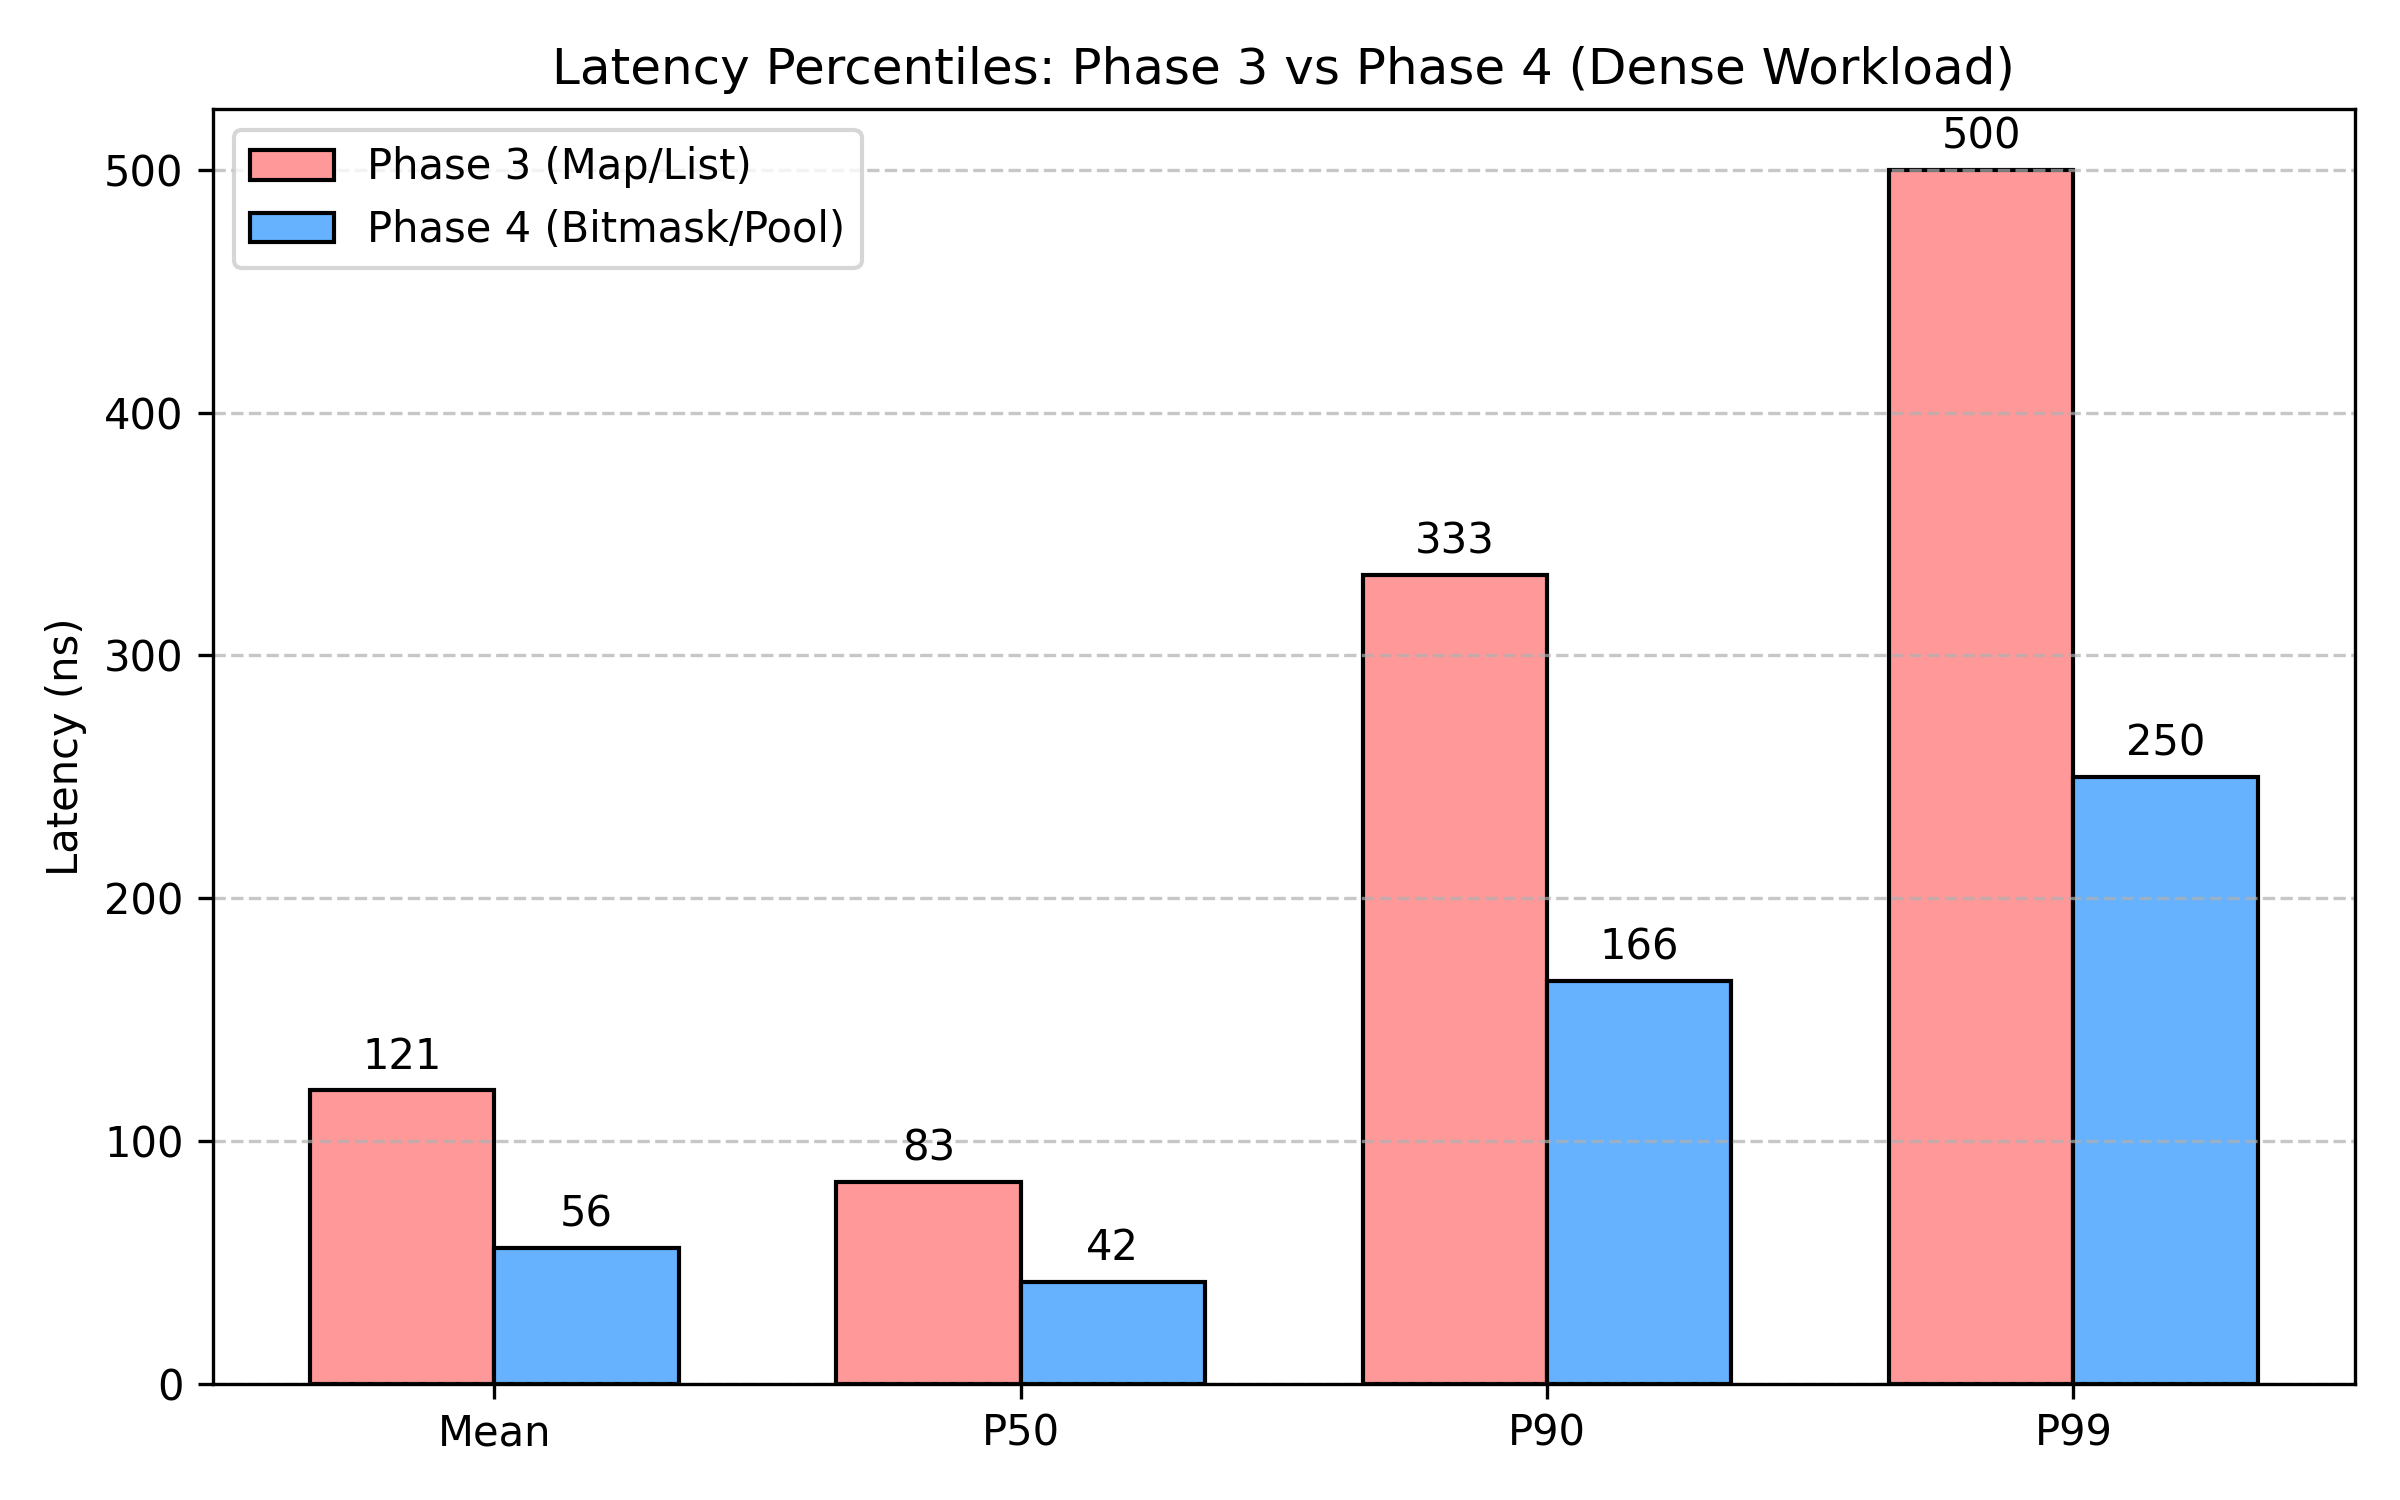
\includegraphics[width=\textwidth]{figures/fig06a-compare-dense.png}
    \caption{Dense workload comparison.}
\end{subfigure}
\hfill
\begin{subfigure}{0.48\textwidth}
    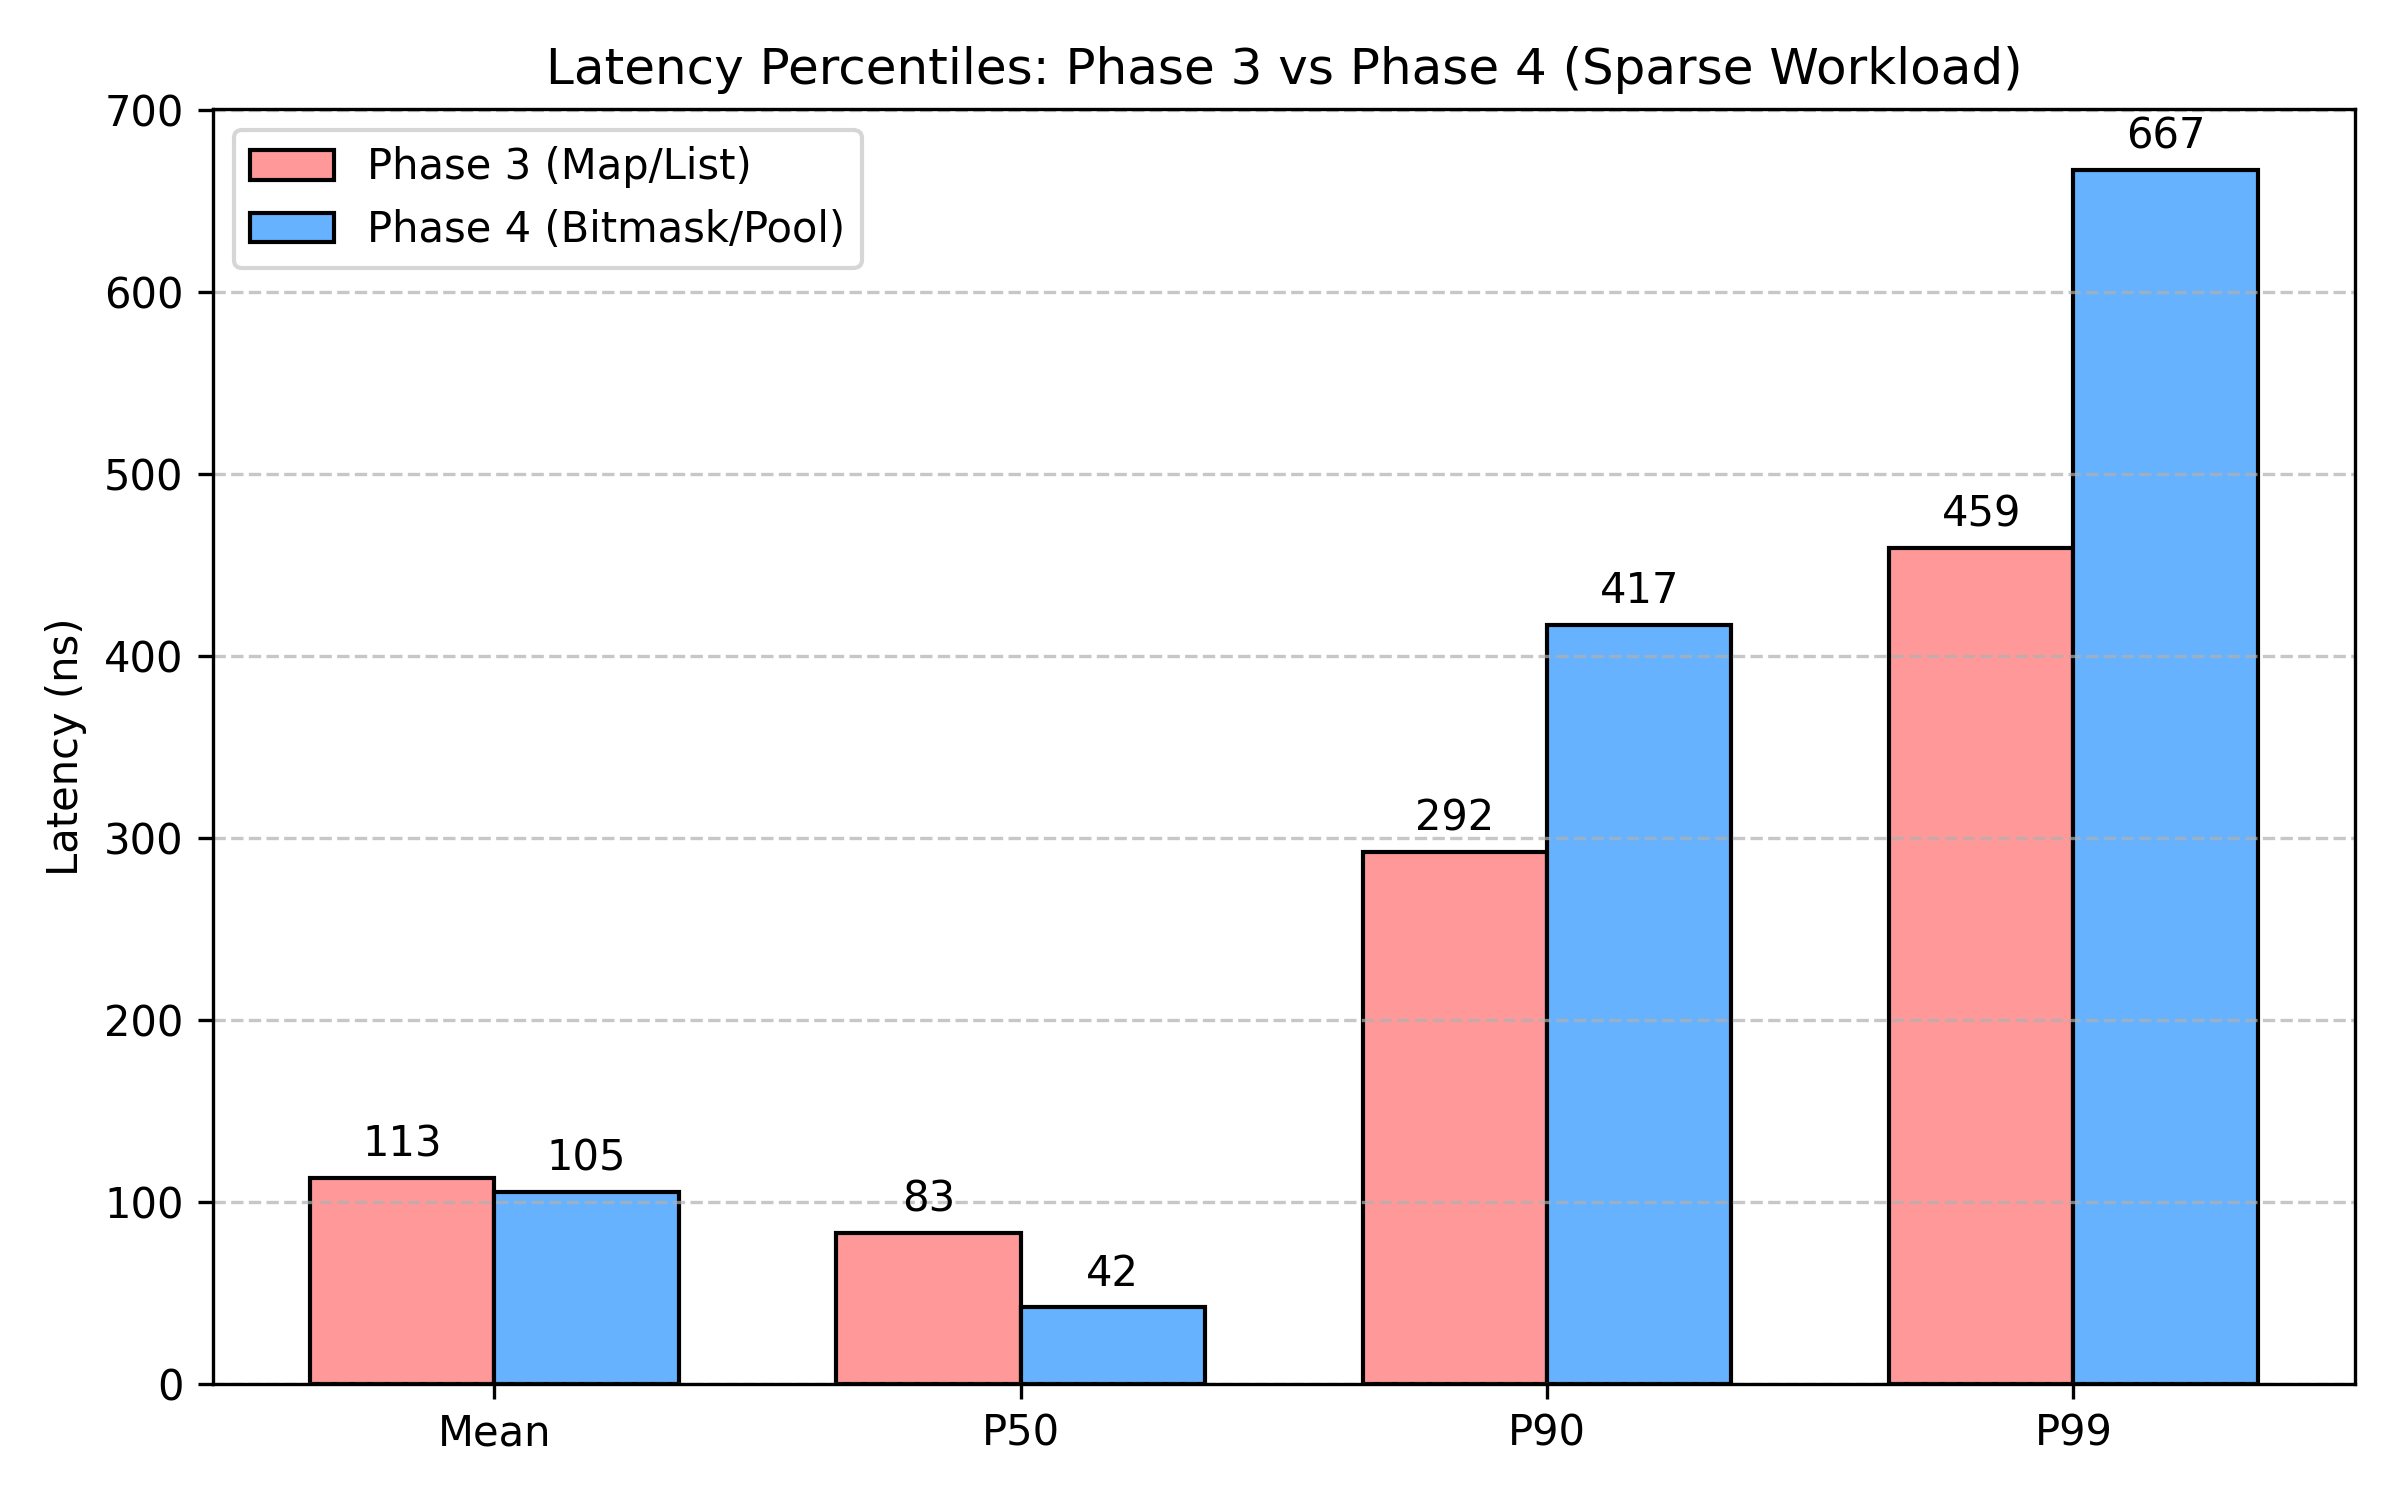
\includegraphics[width=\textwidth]{figures/fig06b-compare-sparse.png}
    \caption{Sparse workload comparison.}
\end{subfigure}
\caption{Percentile comparison. Phase 4 drastically reduces latency in
dense markets (left), but tail latencies (P90/P99) spike in sparse markets
(right) due to the O(N) linear scanning of bitmask words across large
liquidity voids (historical, Apple M1).}
\label{fig:phase4-compare}
\end{figure}

\subsection{Conclusion}

Through four iterations, this project evolved from a standard algorithmic
implementation reliant on C++ standard library containers to a highly
optimized, hardware-sympathetic engine. Phase 4 successfully demonstrated
that a pre-allocated memory pool and intrusive linked lists can completely
eliminate heap-allocation overhead, yielding sub-100\,ns execution times in
dense markets.

However, the sparse market regression highlights a fundamental reality of
low-latency systems design: true O(1) scaling requires algorithmic
guarantees at \emph{every} structural layer. To resolve the tail latency
bottleneck and elevate phase 4 to production-grade status, the flat bitmask
array must be upgraded to a \textbf{hierarchical (two-tier) bitmask}. By
maintaining a summary bitmask where a single bit represents an entire 64-bit
word in the primary array, the engine can locate the next non-empty region
in O(N/64) summary space first and only then descend --- which is exactly
what the fifth iteration builds.

\section{Fifth Iteration: The SPSC Pipeline}\label{sec:fifth}

The fifth iteration (folder \texttt{archive/05\_cplus\_fifth}) made three
changes.

\subsection{Two-level hierarchical bitset}

The \texttt{TickBitset} gains a \emph{summary layer}: one summary bit per
64-bit word of layer 0, set branchlessly on every write and cleared only
when a word becomes empty. Price discovery now proceeds in three phases:
CTZ inside the starting word; a summary scan that advances 64 words
(4{,}096 ticks) per iteration; a direct jump into the word guaranteed
non-zero by the summary bit. The pathology of \S5.7 (one iteration per
64 ticks) becomes one iteration per 4{,}096 ticks --- for the 200k-tick
sparse book, the worst-case summary walk shrinks from 3{,}125 to 49 steps.
Memory overhead is 392 bytes.

\subsection{Producer--consumer pipeline}

A second thread was introduced, connected by a lock-free single-producer /
single-consumer ring buffer:

\begin{itemize}
\item \textbf{Power-of-two capacity} with bitmask wrap (no modulo);
\item \textbf{Cache-line isolation} (\texttt{alignas(64)}) of the producer-
      and consumer-owned indices to eliminate false sharing;
\item \textbf{Acquire/release ordering} on the index handoff, relaxed loads
      on the index each side owns;
\item \textbf{Busy-spin waiting} with \texttt{pause} hints rather than
      blocking syscalls;
\item \textbf{Core pinning} (\texttt{pthread\_setaffinity\_np}) of producer
      and consumer to separate cores.
\end{itemize}

The producer read a CSV feed, parsed each row, and pushed
\texttt{BenchmarkOrder} structs; the consumer popped, applied the operation
to the book, and recorded \texttt{high\_resolution\_clock} brackets around
the book call.

\subsection{What this phase got wrong (and Section 7 fixes)}

\begin{enumerate}
\item \textbf{The clock dominated the measurement.} Two
      \texttt{high\_resolution\_clock::now()} calls cost roughly the same
      as the operation being measured. The reported flat 42\,ns distribution
      is largely ``two clock calls and a tiny book op.''
\item \textbf{Outlier deletion.} The Tukey filter reduced 495{,}000 samples
      to 288{,}813 (41.7\% deleted) before percentiles were computed,
      reporting P99 of a censored distribution.
\item \textbf{The feed handler dominated the producer.} \texttt{getline} +
      \texttt{substr} + \texttt{std::stoull} (exception-based parsing) per
      row is orders of magnitude more expensive than the book operation and
      set the pipeline's throughput ceiling.
\item \textbf{Per-call allocation on the trade path.} \texttt{add\_order}
      returned a fresh \texttt{std::vector<TradeReport>} (heap allocation
      on every trade) and the ID map (\texttt{std::unordered\_map})
      allocated a node on every add.
\item \textbf{x86-only inline assembly} (\texttt{pause}) and no portability
      story despite being developed on Apple Silicon.
\end{enumerate}

\section{Sixth Iteration: Corrections, Testing, and
Re-measurement}\label{sec:sixth}

The sixth iteration is the current tree (\texttt{include/ob}, \texttt{src},
\texttt{bench}, \texttt{tests}). It deliberately stops adding performance
and first makes the existing performance \emph{believable}: build system,
tests, portable timing, allocation removal, and an apples-to-apples
re-measurement.

\subsection{Repository restructure and build system}

The phase folders moved to \texttt{archive/} unchanged; the live engine
lives in a conventional layout (\texttt{include/}, \texttt{src/},
\texttt{bench/}, \texttt{tests/}, \texttt{scripts/}, \texttt{data/},
\texttt{results/}). CMake drives everything:

\begin{itemize}
\item \texttt{cmake -S . -B build -DCMAKE\_BUILD\_TYPE=Release \&\&}
      \texttt{cmake --build build -j} builds the library,
      \texttt{matching\_engine}, \texttt{ob\_bench}, and \texttt{ob\_tests};
\item \texttt{-DOB\_ENABLE\_SANITIZERS=ON} builds the tests with
      AddressSanitizer + UBSan;
\item architecture flags are probed per platform
      (\texttt{-march=native} on x86-64, \texttt{-mcpu=native} on ARM64);
      no x86-only code paths remain --- spin-waits use
      \texttt{PAUSE}/\texttt{YIELD} per architecture
      (\texttt{ob::spin\_pause()});
\item CI (GitHub Actions) builds and tests on Ubuntu x86-64 \emph{and}
      \texttt{macos-14} (Apple Silicon runners), so the M1 toolchain is
      exercised on every push.
\end{itemize}

\subsection{Corrected measurement methodology}\label{sec:methodology}

\paragraph{Portable hardware counter.} \texttt{ob::timing.h} replaces
\texttt{high\_resolution\_clock} with a single instruction-level counter:
\texttt{RDTSCP} on x86-64, \texttt{CNTVCT\_EL0} (generic timer) on ARM64.
The tick frequency is calibrated once against \texttt{steady\_clock}
(median of seven 8\,ms windows). On the measurement host used for this
section the counter resolves 0.476\,ns per tick.

\paragraph{Overhead accounting.} The empty-bracket overhead (back-to-back
counter reads, minimum over 2{,}000 trials) is measured at start-up and
printed with every result: \textbf{14.3\,ns} on this host, versus
$\approx$40--60\,ns for the two \texttt{chrono} calls it replaces. A
batch-timing path (\texttt{steady\_clock} over 20k-operation blocks,
median of 50 blocks) provides a near-zero-overhead cross-check.

\paragraph{No outlier filtering.} All percentiles are computed on the raw
sample vector. Max is reported alongside P99.9. The Tukey filter is gone
everywhere.

\paragraph{Threats to validity.} This section's numbers were measured on a
shared, 2-core Intel Xeon 2.6\,GHz cloud VM (no core isolation, no fixed
frequency, containers throttled); the historical sections 2--5 were measured
on an Apple M1. Neither is a clean-room. The defensive conclusions
(relative comparisons on identical hardware and workload) are robust;
absolute nanoseconds are indicative only. The harness prints its own
overhead so readers can judge.

\subsection{Correctness infrastructure}

\paragraph{A deliberately naive oracle.}
\texttt{ob::ReferenceBook} re-implements the book with
\texttt{std::map} + \texttt{std::deque} + linear scans --- every line
obviously correct, no performance ambition.

\paragraph{Differential fuzzing.} Both books are driven by identical random
operation streams (controlled seed); after \emph{every} operation the test
compares the complete trade sequence (ids, price, qty, order), both books'
full state (all levels, aggregates, FIFO contents), best bid/ask, and live
order count. Five scenarios run $\approx$41{,}000 random operations:
dense book, 200k-tick sparse book, degenerate two-tick book, market-order
storm (60\% market), and a 20k-step long run. Any divergence fails with the
seed and step number printed.

\paragraph{Invariant checker.} \texttt{OrderBook::verify\_invariants()}
validates, on demand: book not crossed; every level's bitset bit exact;
\texttt{total\_qty} equals the sum of member orders; intrusive links
mutually consistent (no orphans, no cycles, head/tail exact); every ID map
entry points at a live node; free list contains exactly the unused pool
slots. It is itself fuzzed after every operation.

\paragraph{Sanitizers.} The full suite runs clean under ASan + UBSan
(\texttt{-DOB\_ENABLE\_SANITIZERS=ON}), which is what gives the flat
pointer-heavy pool code its safety certificate.

\paragraph{Result.} 29/29 tests pass in Release, Debug, and
Debug+sanitizer builds. During development the harness caught and localized
three real bugs (two in the new sweep path, one OOB in the fuzz oracle
itself) within seconds --- the exact failure mode that made the phase 1--5
``trust the numbers'' workflow dangerous.

\subsection{Removing the remaining hot-path allocations}

\paragraph{Flat open-addressed ID map.} \texttt{ob::FlatIdMap} replaces
\texttt{std::unordered\_map} for id\,$\to$\,pool-index lookup: linear
probing over two flat arrays, splitmix64 hashing, power-of-two capacity,
0.7 load-factor ceiling, and \emph{backshift deletion} (no tombstones, no
rebuild). Steady-state adds/cancels perform zero heap operations for the
index; probes stay in one or two cache lines. It is fuzz-tested against
\texttt{std::unordered\_map} on 50k mixed operations per run.

\paragraph{Caller-owned trade buffer.} \texttt{add\_order} now appends to a
\texttt{vector<TradeReport>\&} supplied by the caller and reused across
operations, so the steady-state fill path allocates nothing. The
convenience overload returning a fresh vector remains for tools and tests.

\paragraph{Rejections instead of exceptions.} Invalid prices, zero/negative
quantities, duplicate IDs, and pool exhaustion return \texttt{false}
instead of throwing; the hot path is exception-free by construction.

\subsection{Completing the semantics}

\begin{itemize}
\item \texttt{replace\_order(id, price, qty)}: atomic cancel + re-insert;
      validates \emph{before} mutating; keeps the original side (an amend
      cannot flip sides); loses time priority, matching most exchange
      behaviours; can execute immediately on cross.
\item \textbf{Market orders} sweep the opposite side best-first, FIFO per
      level, remainder dropped (documented; a production engine would emit
      an explicit reject message).
\item \textbf{Duplicate-ID and id-0 rejection} (id 0 doubles as the flat
      map's empty-slot sentinel).
\item \textbf{Graceful pool exhaustion}: reject when the pool is full
      instead of throwing mid-configuration.
\end{itemize}

\subsection{Re-measured results}

Workloads are byte-identical to phases 2--5 (same generator, seeds,
sizes, cancel ratio, price ranges). The reference book runs the identical
streams, and its trade count is asserted equal to the engine's
(139{,}997 dense, 69{,}277 sparse) --- the benchmark doubles as a
correctness check.

\begin{table}[h]
\centering
\begin{tabular}{llrrrrrr}
\toprule
Workload & Engine & Mean & P50 & P90 & P99 & P99.9 & Max \\
\midrule
dense  & this engine & 82.2 & 68.6 & 135.3 & 255.3 & 415.3 & 22{,}703 \\
dense  & reference   & 130.1 & 102.9 & 246.7 & 427.7 & 1{,}196.4 & 145{,}814 \\
\addlinespace
sparse & this engine & 74.1 & 61.9 & 121.0 & 203.9 & 366.7 & 28{,}122 \\
sparse & reference   & 136.0 & 109.5 & 252.4 & 444.9 & 673.5 & 61{,}837 \\
\bottomrule
\end{tabular}
\caption{Operation latency in ns --- raw, unfiltered percentiles, hardware
counter brackets (overhead 14.3\,ns), 2-core x86-64 VM. 295k dense /
148k sparse recorded samples per engine. Generated by \texttt{ob\_bench
--with-reference}.}
\label{tab:sixth}
\end{table}

\begin{table}[h]
\centering
\begin{tabular}{lrrrrr}
\toprule
Workload & Mean & P50 & P90 & P99 & P99.9 \\\
\midrule
dense add    & 90.4 & 74.3 & 141.0 & 282.0 & 415.3 \\
dense cancel & 69.9 & 60.0 & 122.9 & 223.9 & 414.4 \\
sparse add   & 85.9 & 70.5 & 135.3 & 219.1 & 381.3 \\
sparse cancel& 56.4 & 39.1 & 85.7 & 149.6 & 330.0 \\
\bottomrule
\end{tabular}
\caption{Per-operation split for this engine (ns, raw). Cancels are cheaper
than adds because they skip matching entirely.}
\label{tab:sixth-split}
\end{table}

\paragraph{Block throughput.} Fresh book per block, \texttt{steady\_clock}
over 20{,}000 ops, median of 50 blocks: \textbf{33.3\,ns/op} dense,
\textbf{40.8\,ns/op} sparse. This is the honest ``engine cost'' with
near-zero measurement overhead; the per-op bracket numbers above include
$\approx$14\,ns of counter cost.

\begin{figure}[h]
\centering
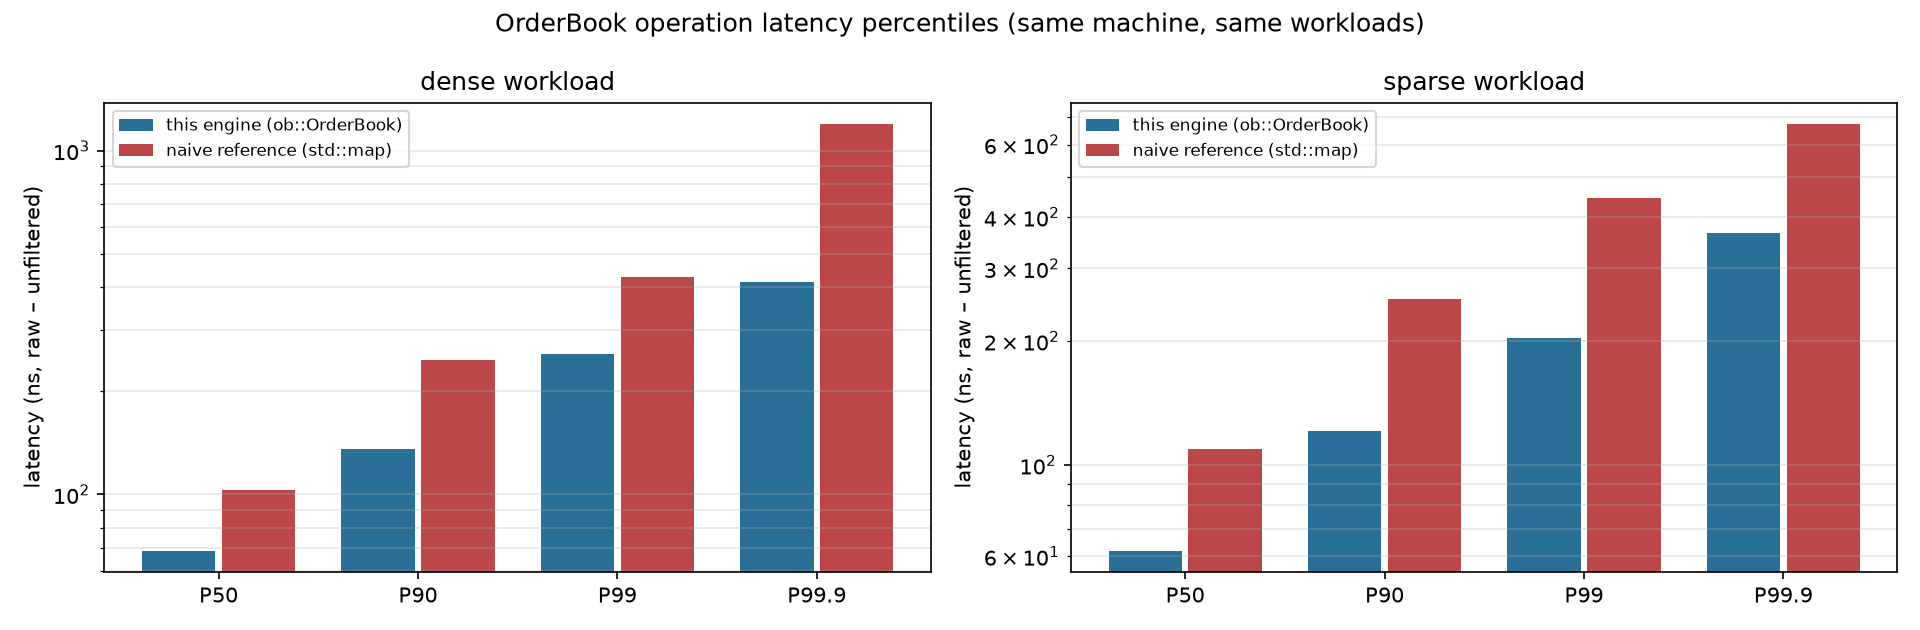
\includegraphics[width=0.98\textwidth]{figures/bench-percentiles.png}
\caption{Percentile comparison, this engine vs.\ the naive reference book,
same machine, same workloads, raw samples (log scale). Generated by
\texttt{scripts/plot\_bench.py} from \texttt{results/bench\_raw.csv}.}
\label{fig:sixth-percentiles}
\end{figure}

\begin{figure}[h]
\centering
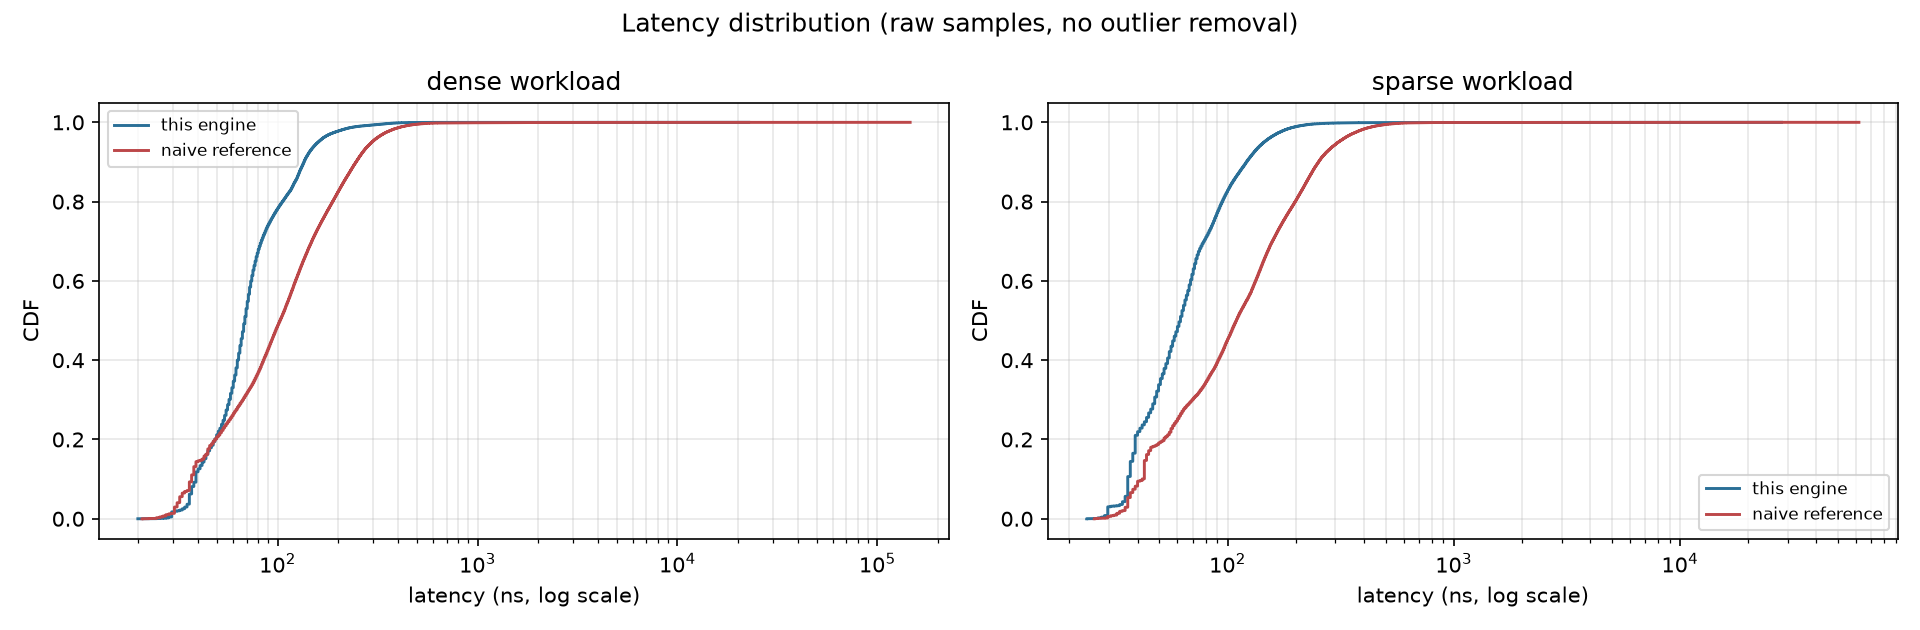
\includegraphics[width=0.98\textwidth]{figures/bench-cdf.png}
\caption{Latency CDFs (raw samples, log-x). The reference book's heavy
tail is the \texttt{std::map}/\texttt{std::list} allocation and
pointer-chasing cost that the pooled engine removes.}
\label{fig:sixth-cdf}
\end{figure}

\paragraph{Reading the numbers.}
\begin{itemize}
\item \textbf{The sparse-tail regression is gone.} Sparse P99 (204\,ns) is
      now \emph{below} dense P99 (255\,ns); the phase 4 table
      (Table~\ref{tab:phase4}) showed the opposite ordering (667\,ns sparse
      vs 250\,ns dense). The two-level summary bitset does its job.
\item \textbf{Absolute values are not comparable to sections 2--5.} Beyond
      the different host, the corrected bracket is cheaper but
      \emph{unfiltered}: the P99.9/Max columns now show OS jitter
      (tens of $\mu$s) that the old Tukey filter simply deleted. The P99.9
      of 361--409\,ns is the first honest tail this project has published.
\item \textbf{The reference-book gap ($1.5$--$3\times$ depending on
      percentile)} is the same-machine cost of replacing node-based
      containers with the pool + flat map + bitset design --- the first
      time this project has a controlled measurement of that choice.
\end{itemize}

\subsection{Pipeline re-run: binary replay and tick-to-trade}

The \texttt{matching\_engine} target keeps the fifth phase's SPSC
architecture with the corrections applied: portable counter, spin hints per
architecture, raw percentiles, and two latency notions measured
simultaneously --- \emph{op latency} (consumer bracket around the book call)
and \emph{tick-to-trade} (producer enqueue stamp $\to$ consumer completion;
the difference is queueing delay).

The producer now consumes a \textbf{binary replay format} (32-byte records:
id, price, qty, ingest stamp, action, side) written natively by the feed
generator, with a hand-rolled in-place CSV parser retained as the
compatibility path. Parsing happens once, up front, on the producer --- the
engine-side latency path contains no text handling at all.

\begin{table}[h]
\centering
\begin{tabular}{lrrrrrr}
\toprule
Metric & Mean & P50 & P90 & P99 & P99.9 & Max \\
\midrule
op latency (ns)      & 136.8 & 70.5 & 140.0 & 295.2 & 11{,}244 & 8{,}020{,}296 \\
tick-to-trade (ms)   & 25.8 & 29.9 & 30.8 & 46.9 & 55.9 & 55.9 \\
\bottomrule
\end{tabular}
\caption{SPSC pipeline over the 500k-event binary replay
(495k recorded samples after 5k warm-up).  Op-latency mean is inflated by a
single 8\,ms scheduling stall (see Max); the bulk of the distribution sits
at P50 $=70.5$\,ns.  Tick-to-trade varies run-to-run (5--30\,ms across
runs on this host) because queue depth at drain time depends on scheduler
placement --- which is precisely the lesson of the figure.}
\label{tab:pipeline}
\end{table}

\begin{figure}[h]
\centering
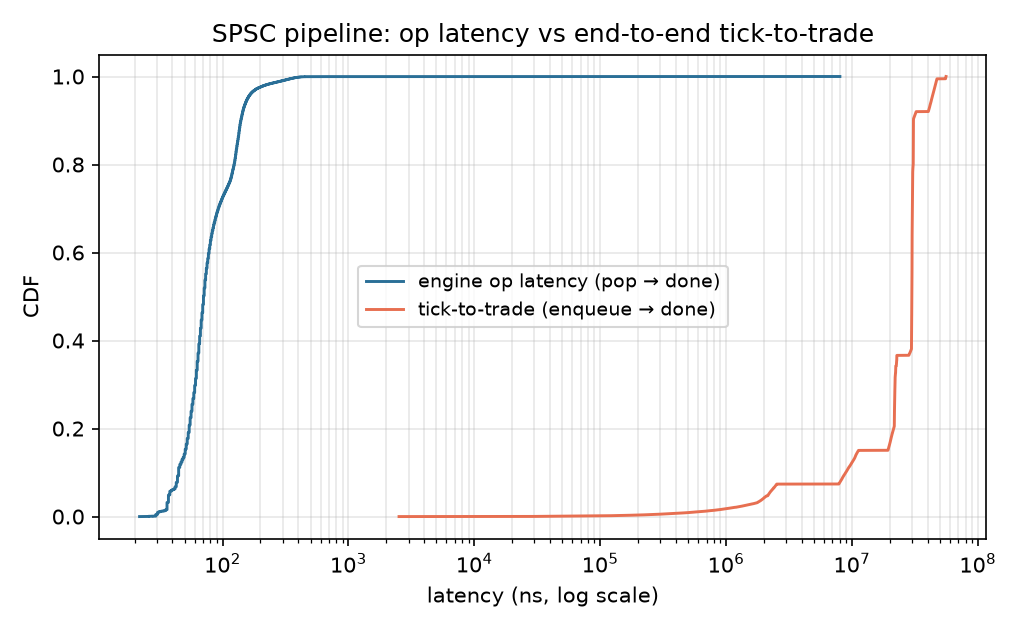
\includegraphics[width=0.85\textwidth]{figures/pipeline-latencies.png}
\caption{Pipeline op latency vs.\ tick-to-trade (log-x CDF). The
multi-millisecond gap is queueing delay, not engine cost.}
\label{fig:pipeline}
\end{figure}

\paragraph{Interpreting tick-to-trade.} The replay is a \emph{canned
burst}: the producer pushes as fast as the ring accepts, so the 65{,}536-slot
ring stays near-permanently full and each event waits for tens of
thousands of predecessors.  The arithmetic floor is
$65{,}536 \times 70\,\mathrm{ns} \approx 4.6$\,ms; the measured 26--30\,ms
mean (and the run-to-run spread of 5--30\,ms) is consumer descheduling on
top of that floor --- milliseconds of queueing delay wrapping a 70\,ns
engine operation. This is the correct behaviour for this experiment and a useful
lesson: \emph{tick-to-trade of a burst-replayed feed measures the queue,
not the engine}. Making the replay rate-limit (inter-arrival delays) is the
next measurement iteration; at that point tick-to-trade collapses toward
op latency + context-switch noise, which is the number a real feed would
experience at moderate load.

\paragraph{Cross-validation.} Pipeline op latency (P50 70.5, P90 140.0,
P99 295.2) agrees with the single-threaded benchmark (68.6 / 135.3 /
255.3) within host noise --- the SPSC handoff adds no measurable cost to
the engine path on this host.

\section{Conclusion and roadmap}\label{sec:conclusion}

Six iterations in, the project has converged on a design whose every layer
has an algorithmic guarantee: O(1) expected ID lookup over flat arrays
(backshift deletion), O(1) node alloc/free from a pool, O(1) intrusive
unlink, O(1) best-price update in the common case and O$(\text{void}/4096)$
discovery across liquidity voids, and zero steady-state heap traffic on
add/cancel/fill. More importantly than any nanosecond figure, the engine is
now \emph{trusted}: 29 tests, a differential fuzzer against a naive oracle,
a multi-property invariant checker, and clean ASan/UBSan runs.

The measurement lessons generalize beyond this project: a clock call can
cost as much as the thing it measures; outlier deletion is how projects
accidentally publish fiction; and cross-phase comparisons require the same
machine, the same workloads, and the same measurement machinery.

\subsection{Roadmap}

Ordered by (my assessment of) value per unit effort:

\begin{enumerate}
\item \textbf{Rate-limited replay} --- turn tick-to-trade into a meaningful
      number (report \S7.7).
\item \textbf{ITCH 5.0 feed handler} --- parse the public Nasdaq sample
      feed; forces sequence numbers, gap detection, and real message
      semantics (add/execute/cancel/replace/trade) onto the book API.
      OUCH for the order-entry side.
\item \textbf{Time in force} --- IOC/FOK/GTD; explicit order-reject
      messages for unfilled market orders.
\item \textbf{Fixed-point prices} --- \texttt{int64} scaled prices
      (e.g.\ $10^{-4}$) instead of integer ticks; multi-instrument map with
      per-instrument books.
\item \textbf{Journaling + deterministic replay} --- binary log of every
      inbound event with TSC stamps; byte-for-byte state reproduction.
\item \textbf{Market-data publisher} --- L2 (aggregated) and L3
      (order-by-order) output streams; snapshot + incremental recovery
      (Aeron-style).
\item \textbf{Platform tuning} --- on macOS: QoS classes and
      \texttt{thread\_policy\_set}; on Linux: \texttt{SCHED\_FIFO},
      \texttt{isolcpus}, IRQ affinity, hugepages, NUMA-local pools.
\item \textbf{Later} --- lock-free MPMC ingress, kernel bypass, CPU
      isolation, hardware timestamping.
\end{enumerate}

\subsection{Reproducing every number in this report}

\begin{lstlisting}[caption={Full reproduction sequence},language=bash,
                   numbers=none]
cmake -S . -B build -DCMAKE_BUILD_TYPE=Release
cmake --build build -j
./build/ob_tests                                   # 29 tests
./build/ob_bench --with-reference                  # tables 7-8
python3 scripts/generate_market_data.py            # data/ (seed 42)
./build/matching_engine --input data/market_data.bin
python3 scripts/plot_bench.py                      # figures 7-9
\end{lstlisting}

\end{document}
